\documentclass[11pt]{article}
\usepackage{geometry}
\geometry{
 a4paper,
 total={210mm,297mm},
 left=25mm, 
 right=25mm,
 top=25mm,
 bottom=25mm,
 }
 
\usepackage[english]{babel}
\usepackage[utf8x]{inputenc}
\usepackage{amsmath}
\usepackage{graphicx}
\usepackage{multicol}
\usepackage{ragged2e}
\usepackage{tocloft}
\usepackage{gensymb}
\usepackage{siunitx}
\usepackage[hypcap]{caption}
\usepackage{capt-of}
\usepackage{setspace}
\usepackage[parfill]{parskip}
\usepackage{amssymb}
\usepackage{textcomp}
\usepackage{float}
\floatstyle{plain}
\usepackage{color}
\usepackage{epstopdf}
\usepackage{natbib}
\usepackage{hyperref}
\hypersetup{
    colorlinks=true,
    linkcolor=black,
    filecolor=magenta,      
    urlcolor=cyan,
    citecolor=black
}
\urlstyle{same}
\usepackage{cleveref}
\usepackage{lastpage}
\usepackage{fancyhdr}
\usepackage{graphicx}

\usepackage[normalem]{ulem}
\useunder{\uline}{\ul}{}
\usepackage{pdflscape}
\usepackage{multirow}
\usepackage[table,xcdraw]{xcolor}
\usepackage{hhline}


%abstract setup
\renewenvironment{abstract}
 {\hspace{.8cm}
  {\bfseries\huge\abstractname}
  \list{}{
    \setlength{\leftmargin}{.95cm}%
    \setlength{\rightmargin}{\leftmargin}%
  }%
  \item\relax}
 {\endlist}

%random things needed
%\renewcommand{\cftsecleader}{\cftdotfill{\cftdotsep}} %let the content table have dots to number
\linespread{1.6}  %one and half is 1.3, doublespacing is 1.6
\frenchspacing


\begin{document}

\begin{titlepage}
	\centering
	\topskip0pt
	\vspace*{\fill}
	{\huge\bfseries Temporal turnover of plant-pollinator interaction networks \par}
	\vspace{2cm}
	{\Large \textsc{Lim} Jia Le  {    }  CID: 00865029}
	\\ 	\vspace{0.5cm}
	{Department of Life Sciences, Imperial College London, \\Silwood Campus, London, U.K.} \\ \vspace{0.5cm}
	{Submitted in part fulfilment of the requirements for the \\ Bachelor of Science degree in Biology with German for Science \\ at Imperial College London.} \\
	\vspace*{\fill}
	{\large Supervised by\par
	Dr.~Samraat \textsc{Pawar}}
	\vfill
% Bottom of the page
	{\large Last updated: \today\par}
\end{titlepage}

% abstract page
\newpage
\pagenumbering{gobble}
\vspace*{\fill}
\begin{abstract}  %140 words
\vspace{1.5cm}
\doublespacing
Plant-pollinator interactions are ecologically significant and economically important. Although it is widely agreed that climate affects plant physiology and flowering phenophases, little is known about how or if these responses influence plant-pollinator interactions. Most temporal network studies have focused on the impact of the climate on network structure and robustness but have failed to draw a clear link between climate change and species interactions. In this study, I develop a framework for investigating the influence of climatic factors on interaction turnover using two datasets collected in the Cerrado and present evidence that month-to-month interaction turnover is surprisingly and consistently high. Moreover, this study shows that temperature positively correlates with plant turnover during wet seasons in the Cerrado. Furthermore, plant turnover is a strong predictor of interaction turnover, hence suggesting that elevated global temperatures may drive an increase in temporal interaction turnover. 
\end{abstract}
\vfill

% contents page
\newpage
\pagenumbering{gobble}
\vspace*{\fill}
\tableofcontents 
\vspace*{\fill} 
\thispagestyle{empty}

\doublespacing

% abbreviations page
\newpage 
\vspace*{\fill}
{\huge\bfseries Abbreviations} \\
\\
\\
\begin{table}[h]
\centering
\large
\setstretch{2}
\label{my-label}
\begin{tabular}{lll}
BBG:            &  & Bras\'ilia's Botanical Garden Protected Area             \\
IBGE:           &  & Reserva Ecol\'ogica do IBGE                              \\
$\beta_{int}$:   &  & Interaction turnover                                     \\
$\beta_{rw}$:    &  & Interaction rewiring                                     \\
$\beta_{st}$:    &  & Contribution of species turnover to interaction turnover \\
$\beta_{S}$:     &  & Species turnover                                         \\
$\beta_{Bee}$:   &  & Bee turnover                                             \\
$\beta_{Plant}$: &  & Plant turnover                                          
\end{tabular}
\end{table}
\vfill

% Page number
\newpage
\pagestyle{fancy}
\fancyhf{}
\renewcommand{\headrulewidth}{0pt}
\rfoot{Page \thepage \hspace{1pt} of \pageref{LastPage}}
\pagenumbering{arabic}

%%% Start writing
\section{Introduction} % 985 words

Plant-pollinator interactions contribute significantly towards the diversity of ecosystems by maintaining species-level fitness and community composition in plants~\citep{Olesen2008}. Moreover, pollination services constitute a major part of our global economy by supporting the crop industry and contributing towards food security. This field of study has therefore attracted much attention in recent years~\citep{Allsopp2008}. \\
\\
Studies of plant-pollinator networks have provided much insight into the structure of ecosystems and their function. In these networks, a link is created between a pollinator and a plant when a pollinator visits the flowers of the plant. Both species are represented by the nodes of the networks, where every link between nodes constitutes a pollination event~\citep{Poisot2012}. \\
\\
Nonetheless, previous studies have typically depended upon a static picture of plant-pollinator networks and ignored the dynamic nature of interactions. Recently, compelling evidence has surfaced, demonstrating that interaction networks vary between days, weeks, within seasons and even across decades or centuries~\citep{Olesen2008, Burkle2013, Yeakel2014, CaraDonna2017}. However, the significant amount of sampling effort required to build multiple networks has resulted in insufficient studies on temporal networks~\citep{Burkle2011}.\\
\\
Research on temporal plant-pollinator networks has likewise been largely restricted to peak flowering seasons and temperate ecosystems. These studies have mainly focused on the robustness, stability and structure of temporal networks and the factors that constrained interactions across time~\citep{BASILIO2006, Olesen2008, CaraDonna2017}. However, relatively little is known about the drivers of high temporal variability of interactions~\citep{Burkle2011}.\\
\\
Understanding the factors that drive interaction turnover can provide new insight into the impact of climate change on plant-pollinator networks. Elevated global temperature results in drastic shifts in flowering, which can lead to disruptions of spatial and temporal co-occurrences of flowers and pollinators in temperature regions~\citep{Schweiger2010}. Moreover, even if climate change causes subtle differences in plant or pollinator phenology, these minute changes could affect each other, eventually significantly influencing interaction networks. For example, changes in plant physiology could lead to reduced pollinator reproduction, which could indirectly cause reduced pollination visits in a positive feedback loop, hence resulting in an amplified effect of climate change on plant-pollinator interactions~\citep{Scaven2013}. \\
\\
In the tropics, most pollinators are active for periods longer than the flowering periods of most plants~\citep{Biesmeijer2006}. Plant phenology shifts may hence not have the same impact on species interactions as in the temperate regions, where most interaction network studies have been conducted. Thus, the direct influence of rising temperatures and harsher weather conditions on plant-pollinator interactions in tropical regions remains unclear~\citep{Schweiger2010}.  \\
\\
The greatest biodiversity in the world can be found in the tropics~\citep{Brown2014}. Understanding the variability of interactions in these habitats is hence crucial in maintaining plant-pollinator interactions and species richness in the tropics. In this study, I focus on temporal interaction networks in the Cerrado; a neotropical habitat characterised by drastic seasonal changes between dry and rainy seasons~\citep{Kricher2011}.\\
\\
%The Brazilian Cerrado is a seasonally dry savanna that consists of a variety of pollinators with bees as its major pollinating agent. Many Cerrado bees are active throughout the year as they live in colonies or produce multiple generations annually. In contrast, seasonal changes in precipitation can constrain dry season flowering in plants with shallow root systems, such as herbs and shrubs~\citep{Gibbs2002, TobyPennington2006, Gottsberger2006}. 
Besides being a highly seasonal habitat, the Cerrado acts as an important model system for interaction network studies as it sustains a significant percentage of the Neotropical angiosperm diversity. The Cerrado is the second largest tropical biome in South America and is viewed as one of the most threatened tropical ecosystems due to excessive deforestation and poor conservation policies, which have already caused more than 50 \% of its area to be degraded. Unfortunately, data of the region is scarce and the ecological networks of this region are poorly understood~\citep{Myers2000, KLINK2005}. Thus, a better understanding of the interaction networks of this region will significantly help conservation efforts in the Cerrado.\\
\\
In this study, two different datasets collected in the tropical Cerrado habitat were used to investigate temporal interaction turnover. To the best of my knowledge, this is the first study to investigate the effect of climatic factors on temporal interaction turnover. Here, I report that temporal interaction turnover is surprisingly and consistently high in the Cerrado. Moreover, plant turnover is a strong driver of interaction turnover. Temperature in the wet season is also positively correlated with plant turnover, indicating that a rise in temperature may indirectly increase interaction turnover. 

\newpage
\section{Materials and Methods} % 1549 words

To address the questions stated above, I develop a framework for investigating the influence of climatic factors on interaction turnover~(\autoref{fig: flowchart}). Firstly, differences between subsequent temporal networks, also known as $\beta$-diversity, were quantified using a number of $\beta$-dissimilarity measures. These measures reflect interaction, species, plant and bee species changes over time. Correlations between $\beta$-dissimilarity measures were then investigated and compared to theoretical and previously published trends. Lastly, to provide a macroscopic view, relationships between climatic factors and temporal dissimilarity in plant communities were examined.\\

\begin{figure}[h]
  \centering
    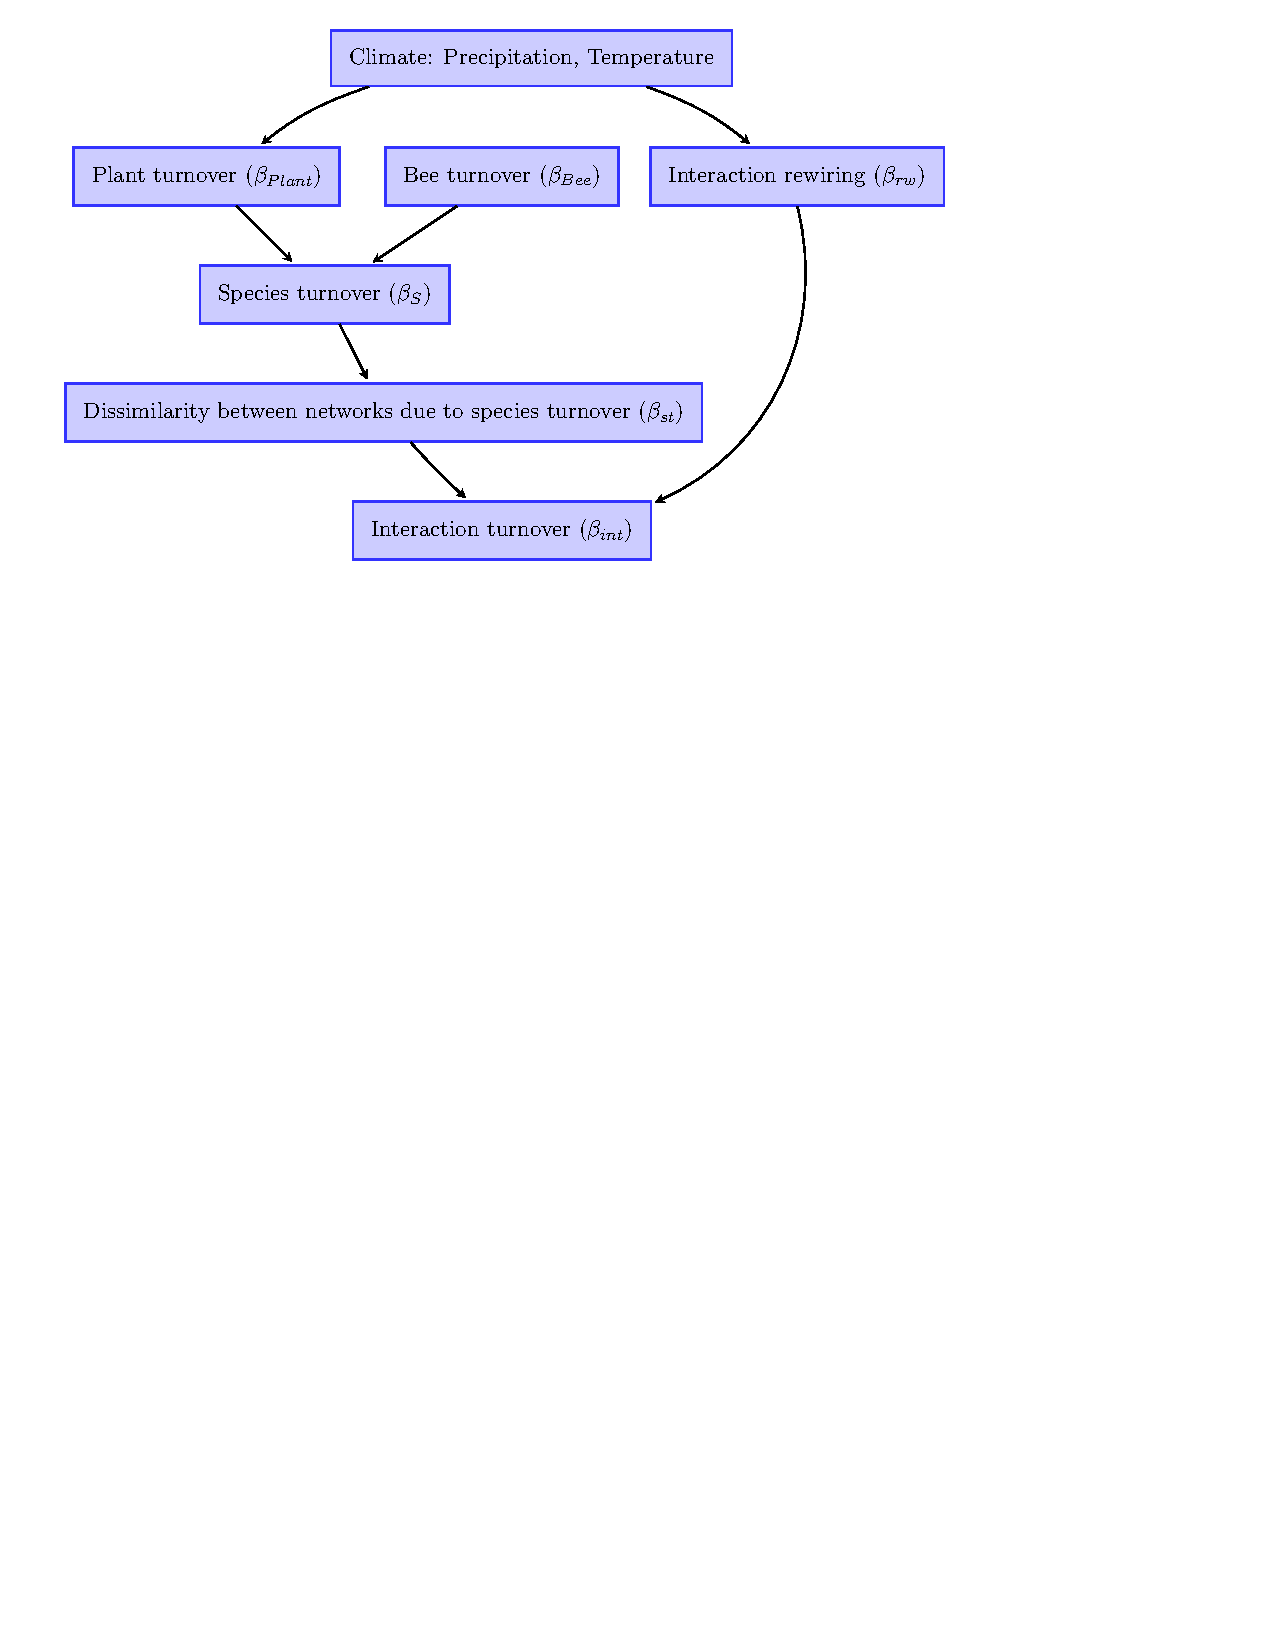
\includegraphics[width=0.8\textwidth]{flowchart.pdf} \\
    \captionof{figure}{\setstretch{1.3} Framework demonstrating the effect of climatic factors on the different measures of turnovers.}
    \label{fig: flowchart}
\end{figure}

\subsection{Study area}
The Cerrado spans across most of Central Brazil while extending marginally into Bolivia and Paraguay. It comprises of vegetation ranging from open grasslands to scrublands with a sparse distribution of trees, and smaller regions of gallery and close canopy forests. These patches exist side-by-side, resulting in a highly heterogeneous ecosystem~\citep{Gottsberger2006}. \\
\\
Plant-pollinator interactions were surveyed in the Protected Area of the Jardim Bot\^anico de Bras\'ilia (Bras\'ilia's Botanical Garden Protected Area; hereafter `BBG') and in the Reserva Ecol\'ogica do IBGE (hereafter `IBGE') . The two study sites are located on the Brazilian plateau (1,100m a.s.l.), within the federally protected conservation site ``APA-Gama-Cabe\c ca-de-Viado'', located approximately 30km south of Bras\'ilia (15\degree56'S, 47\degree53'W). This region is characterized by a well-defined wet summer season that lasts from November until March followed by a dry winter period that extends from May until September~\citep{Gottsberger2006a}.\\
\\
The IBGE site consisted of a 8-hectare plot (200 x 400m) covered with mainly grasses mixed with herbaceous plants and shrubs, with a sparse distribution of lianas and trees. In contrast, the BBG site comprised of a denser type of vegetation with a predominance of large shrubs, lianas, and trees~\citep{Eiten1972}.

\subsection{Sampling methods and species identification}
Bees are the predominant pollinators in the Cerrado ($\sim$70\%) followed by moths ($\sim$12\%), hummingbirds ($\sim$3\%), bats, ($\sim$2\%) and beetles ($\sim$2\%)~\citep{Oliveira2002, Gottsberger2006a, Cappellari2011}. Hence, this study focused only on bee-flower interactions. A plant or pollinator species was included in the surveys only if the flowering plant received visits or if the bee was seen foraging on flowers. For every interaction observed, the plant was tagged with a unique identification number, photographed and vouchered. Plant vouchers were identified by using comparative herbarium material, a checklist of local angiosperms and local botanical expertise (Refer to \hyperref[sec: acknowledgements]{Acknowledgements}).  In both sites, bees were collected with an entomological net and killed either in individual vials with paper pellets moistened with ethyl acetate or frozen after each observation. Insect vouchers were thereafter mounted, preserved, and identified to species level by comparison with reference collections, taxonomic literature, local records~\citep{Moure1962, Silveira2002, Michener2007, Moure2007} and by local entomological experts (Refer to \hyperref[sec: acknowledgements]{Acknowledgements}). \\
\\
The BBG area was sampled weekly (0730h to 1700h) by M. C. Boaventura from June 1995 to June 1997 using two predefined transects (5,280m and 4,130m in length) located 4 km apart~\citep{Boaventura1998}. Sampling in this site totaled 125 days over 25 months (mean = 5 days/month). Interactions involving the introduced honey bee (\textit{Apis mellifera}) were not included in the BBG data set. The IBGE study site was sampled by S.C. Rabeling by walking transects covering the entire area for a full day (0800h to 1700h) at a weekly basis from November 2008 to October 2009. In total, there were 47 sampling days over a 12-month period (mean = 3.91 days/month). 
% why wasnt the honey bee added

\subsection{Climate information}

Data from the IBGE's weather station was used to obtain monthly median temperature and precipitation sum for the past 30 years (1980 - 2010). Median temperature was adopted as monthly distributions of daily average temperatures were skewed. Humidity was not considered as only relative humidity data of IBGE was made available.\\
\\
Monthly precipitation sum from June 1995 to June 1997 ranged from 0 mm to 358 mm while median temperatures varied between 18.4\degree C to 23.5\degree C. From October 2008 until September 2009, monthly precipitation sum ranged from 0 mm to 270.6 mm with median temperatures of 18\degree C to 24\degree C~(\hyperref[table: climate]{Table S\ref{table: climate}}). For analytical purposes, the interactions recorded in the transitional months of April and October were assigned to the dry and rainy seasons respectively. Turnovers between networks of September and October and those between networks of March and April were similarly designated to the dry and rainy seasons respectively. Periods specified for each season are in concordance with patterns reported for other Cerrado areas~\citep{Gottsberger2006a}. 

\subsection{Data analysis}
Due to temporal and spatial differences between the BBG and IBGE datasets, the two datasets were analysed separately. 

\subsubsection{Month-to-month turnover}
Bee-flower interaction turnover is calculated using the Whittaker's presence-based dissimilarity measure~\citep{Whittaker1960}: 
\begin{align}
	\beta_{int} & = \frac{a + b + c}{(2a + b + c)/2} - 1 
\label{eq: dissimilarity}
\end{align}
where interaction turnover (i.e. interaction dissimilarity or interaction $\beta$-diversity; $\beta_{int}$) reflects the differences, or dissimilarity, of interactions between two successive monthly networks. $a$ represents the number of interactions present in both networks while b and c are the number of unique interactions present in each of the two networks respectively~\citep{Poisot2012}. \\
\\
The Whittaker's index was chosen as it is most commonly used for presence-absence data. Moreover, it does not require additional information such as abundance of species in Cerrado, in which data is scarce, and is relatively more robust than other $\beta$-dissimilarity indexes when dealing with heterogeneous dataset sizes~\citep{Koleff2003, Poisot2012}. \\
\\
$\beta_{int}$ can be partitioned into two components; network dissimilarity due to species turnover ($\beta_{st}$) and interaction rewiring between shared species of networks ($\beta_{rw}$):
\begin{align}
	\beta_{int} & = \beta_{st} + \beta_{rw} 
\label{eq: interaction}
\end{align}
\vspace{0.1cm} \\
In theory, $\beta_{int}$ and $\beta_{st}$, but not $\beta_{rw}$, covary with species turnover, $\beta_{S}$, where $\beta_{S}$ reflects the differences between species composition of two networks~\citep{Poisot2012}. In this study, $\beta_{S}$ can be driven by either plant turnover ($\beta_{Plant}$) or bee turnover ($\beta_{Bee}$). \\
\\
\\
$\beta_{rw}$, $\beta_{S}$, $\beta_{Plant}$ and $\beta_{Bee}$ are calculated using \hyperref[eq: dissimilarity]{Equation \ref{eq: dissimilarity}}, where $a$ refers to the number of items present in both networks and $b$ and $c$ refer to the number of unique items present in each of the two networks~(\autoref{table: dissimilarity}, \hyperref[fig: calculationex]{Figure \ref{fig: calculationex}}). $\beta_{st}$ is obtained by subtracting $\beta_{rw}$ from $\beta_{int}$~(\hyperref[eq: interaction]{Equation \ref{eq: interaction}}). The dissimilarity measure takes the value of 0 when two networks are identical and the value of 1 when two networks do not share any items in common~\citep{Poisot2012, CaraDonna2017}. \\

%%%%%%%%%%%%%%%%%%%%%%%%%%%%%%%%%%%%%%%%%%%%%%
\begin{table}[h]
\captionof{table}{Measures of network dissimilarity. \\ \doublespacing\footnotesize The contribution of species turnover to interaction turnover is illustrated indirectly by the fraction of interaction turnover due to species turnover alone ($\beta_{st}$). Dissimilarity measures are calculated using the respective items and ~\autoref{eq: dissimilarity}.}
\label{table: dissimilarity}
\doublespacing
\resizebox{1.07\textwidth}{!}{%
\begin{tabular}{llll}
\hline
\rowcolor[HTML]{FFDA6C} 
Measure & Definition & Items & Reference \\ \hline
$\beta_{int}$ & \begin{tabular}[c]{@{}l@{}}Dissimiliarity of interactions; \\ Interaction turnover\end{tabular} & All interactions & \begin{tabular}[c]{@{}l@{}}\cite{Canard2011}; \\ \cite{CaraDonna2017}  \end{tabular} \\

\rowcolor[HTML]{FFF9F1} 
$\beta_{rw}$ & \begin{tabular}[c]{@{}l@{}}Dissimilarity of interactions between species present in both networks; \\ Interaction rewiring\end{tabular} & \begin{tabular}[c]{@{}l@{}}Interactions of \\ shared species\end{tabular} & \begin{tabular}[c]{@{}l@{}}\cite{Canard2011};\\ \cite{CaraDonna2017} \end{tabular} \\

$\beta_{st}$ & Dissimilarity of interactions due to species turnover & \autoref{eq: dissimilarity} & \cite{Poisot2012}  \\

\rowcolor[HTML]{FFF9F1} 
$\beta_{st}$/$\beta_{int}$ & Contribution of species dissimilarity to dissimilarity of interactions &  & \cite{Poisot2012} \\

$\beta_{S}$ & \begin{tabular}[c]{@{}l@{}}Dissimilarity in the species composition of both networks; \\ Species turnover\end{tabular} & Species identity & e.g. \cite{Koleff2003} \\

\rowcolor[HTML]{FFF9F1} 
$\beta_{Bee}$ & \begin{tabular}[c]{@{}l@{}}Dissimilarity in the bee composition of both networks; \\ Bee turnover\end{tabular} & Bee identity & This study \\

$\beta_{Plant}$ & \begin{tabular}[c]{@{}l@{}}Dissimilarity in the plant composition of both networks; \\ Plant turnover\end{tabular} & Plant identity & This study \\ \hline
\end{tabular}%
}
\end{table}

%%%%%%%%%%%%%%%%%%%%%%%%%%%%%%%%%%%%%%%%%%%%%%

\subsubsection{Correlation}
As turnover measures are not normally distributed, the non-parametric Spearman's rank correlation test from the python package SciPy was utilised to investigate the relationships between the different dissimilarity measures as well as the associations of climatic factors and dissimilarity measures~\citep{Dehmer2011}. \\
\\
A Monte Carlo procedure was then used to generate p-values for correlation tests. p-values of Spearman's test deviate away from actual p-values due to turnovers being dependent variables~(\hyperref[table: turnoverspearman]{Table S\ref{table: turnoverspearman}}). Randomised sets of bees and plants were drawn across the dataset to form $10^{5}$ simulated networks for each month. Correlation coefficients between turnover measures for each simulation were thereafter calculated. Number of bees, plants and interactions as well as connectance of each monthly network in simulations were kept constant. p-values were obtained by dividing the total number of simulations with a correlation coefficient higher than the value obtained in either the BBG or IBGE dataset by $10^{5}$.

\subsubsection{Climate}
The two seasons exhibit different temperature and precipitation ranges, resulting in seasonal interactions~(\hyperref[fig: seasonalnetworks]{Figure \ref{fig: seasonalnetworks}}). To investigate whether precipitation and/or temperature affects turnovers, two climatic models were utilised in this study. \\
\\
The first model uses the differences between precipitations or temperatures of two subsequent months as the explanatory variable of turnover (hereafter known as the difference model). The alternative hypothesis of the difference model assumes that networks at a particular temperature and precipitation level are static and do not experience changes as long as climatic factors remain constant. When two networks are at the same temperature and precipitation level, interaction turnover equals to zero. Interaction turnover increases as the temperature or precipitation level difference between networks increases.\\
\\
The second model uses the average of precipitations or temperatures of two subsequent months as the explanatory variable of turnovers (hereafter known as the average model). The average model postulates that two networks with identical climatic factors will yield a particular turnover rate. Interaction turnover increases as the temperature or precipitation level of networks increases.\\
\\
To compare the two climatic models, linear regression was used to fit $\beta_{Plant}$ and $\beta_{int}$ against precipitation, temperature and season and their interactions. Due to its small size, the IBGE dataset was not utilised in model fitting. The more explanatory model was thereafter used to fit turnovers against climatic factors within seasons to prevent overfitting and to minimise multicollinearity.
% climate models comparison

\newpage
\section{Results}
\label{sec: Results} % 1336 words
\subsection{Community composition}
111 species of bees and 93 species of plants were recorded over the 12-month study period at IBGE. In total, 968 bee-flower interactions, which comprised of 434 unique interactions, were observed. The bee community composition in IBGE was similar to those previously observed in other Cerrado areas~\citep{Silveira1995, Pinheiro-Machado2002} with Apidae being the richest group (77 spp.) followed by Halictidae (19 spp.), Megachilidae (13 spp.), Andrenidae (1 sp.), and Colletidae (1sp.). Plant species recorded at this site consisted of mainly herbs and shrubs and belonged to 24 families, with the most species rich group being Fabaceae (18 spp.). \\
\\
Between June 1995 and June 1997, 1050 unique interactions and 1616 visitation events between 203 bee species and 182 plant were recorded in the \textit{cerrado sensu strictu} area of BBG. Although the BBG area contained a more species rich pollinator community, bee families were present in comparable proportions as those observed in IBGE: Apidae (115 spp.), Halictidae (38 spp.), Megachilidae (27 spp.), Colletidae (3 spp.), and Andrenidae (1 sp.). Plants recorded in BBG represented 41 families, consisting of mostly shrubs, some trees, and a few herbs. Similar to IBGE dataset, Fabaceae was the most species rich group in this area (31 spp.), followed by Asteraceae (20 spp.) and Malpighiaceae (17 spp.). 
% generalised?

\subsection{Month-to-month turnover}
\label{subsec: turnover} 

% percent of interactions present in more than 6 monthly interactions -> networks figures
Interaction turnover, $\beta_{int}$, is consistently high, ranging from 0.747 to 1~(\hyperref[table: turnovers]{Table S\ref{table: turnovers}}, \hyperref[fig: turnovertimeplotold]{Figure \ref{fig: turnovertimeplotold}}, \hyperref[fig: turnovertimeplotnew]{Figure \ref{fig: turnovertimeplotnew}}). Surprisingly, only 8.19\% and 4.83\% of all unique interactions appeared in three or more monthly networks at the BBG and IBGE site respectively~(\autoref{fig: networks}).\\
\\
As expected, $\beta_{int}$ is positively correlated with $\beta_{S}$~(BBG: $r_{s}$=0.698, $p$=0.0308; IBGE: $r_{s}$=0.809, $p$=0.0123)(\autoref{fig: turnoversbivariate}) as an increase in species turnover, $\beta_{S}$, will result in an elevated $\beta_{int}$. At both sites, $\beta_{int}$ is significantly and positively correlated with $\beta_{Plant}$ (BBG: $r_{s}$=0.822, $p$=0.00008; IBGE: $r_{s}$=0.773, $p$=0.0118), suggesting that $\beta_{Plant}$ drives $\beta_{int}$~(\autoref{fig: plantturnover}).\\


%%%%%%%%%%%%%%%%%%%%%%%%%%%%%%%%%%%%
\newpage
\begin{landscape}
\vspace*{\fill}
\begin{figure}[H]
  \centering
    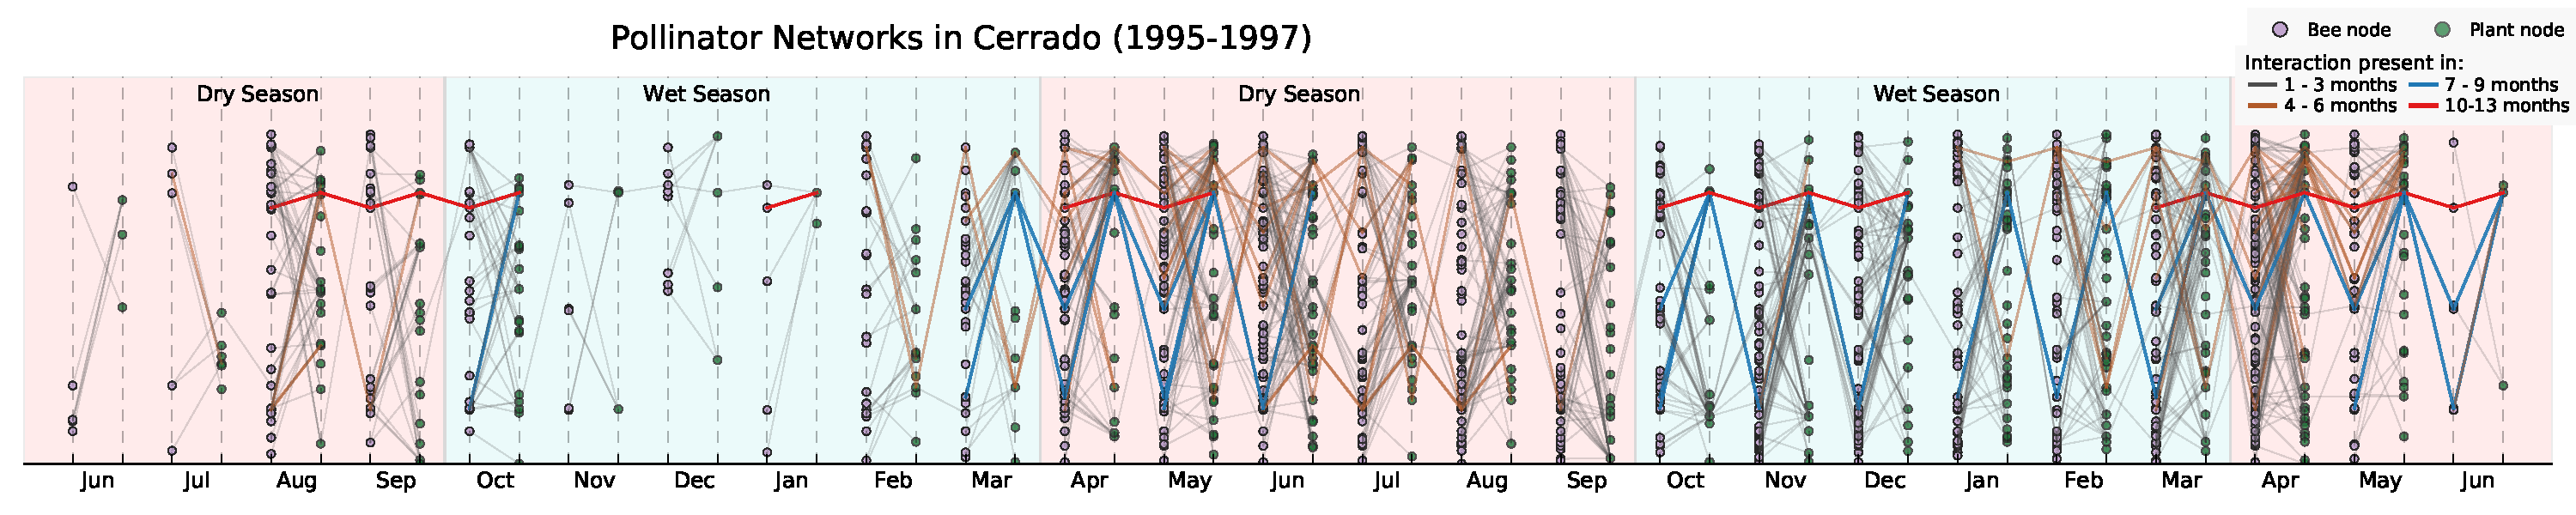
\includegraphics[width=260mm]{network(old).pdf} \\
    \vspace{1cm}
    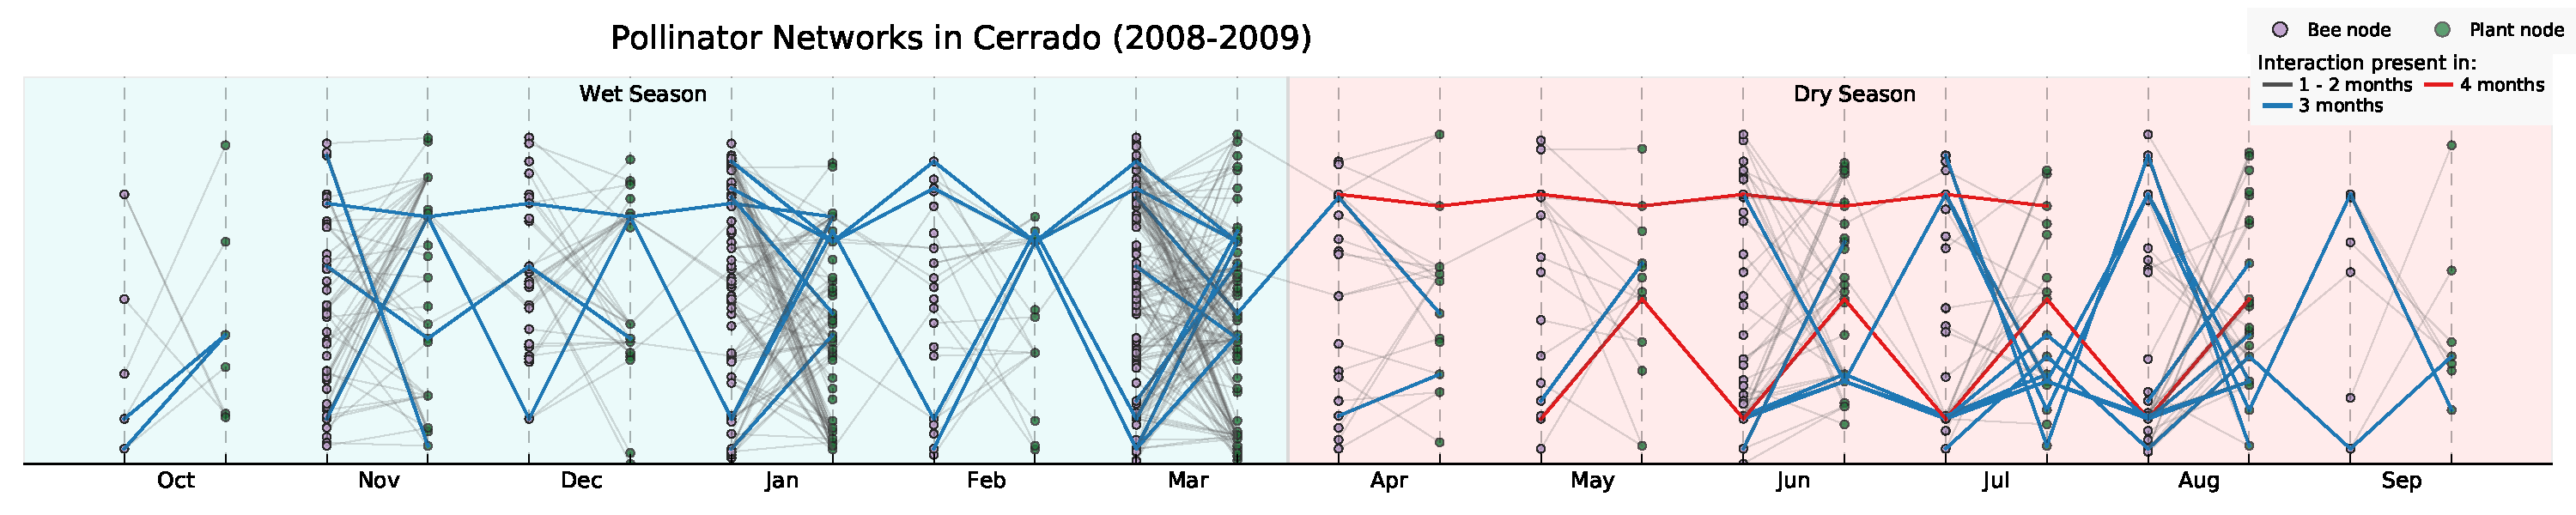
\includegraphics[width=260mm]{network(new).pdf}
    \captionof{figure}{\setstretch{1.3} Monthly bee-plant networks from Jun 1995 to Jun 1997 (BBG site) and from Oct 2008 to Sep 2009 (IBGE site).\\ \footnotesize Every node in a monthly network represents a distinct plant or bee species. Each link between plant and bee nodes represent a unique pollination visit in the corresponding month. Links between monthly networks show interactions recorded in both monthly networks. Background of plot is colour-coded to reflect the seasons: blue - wet season; red - dry season. Faded areas bound the pollinator networks of each month, while darker areas highlight the links present between monthly networks. Colour of links represent the number of monthly networks in which the interaction was found. (BBG: Total no. of unique interactions: 1050, No. of interactions present in 4-6 months: 20, 7-9 months: 3, 10-13 months: 1; IBGE: Total no. of unique interactions: 434, No. of interactions present in 1-2 months: 414, 3 months: 18, 4 months: 2)}
    \label{fig: networks}
\end{figure}
	\vspace*{\fill}
\end{landscape}
%%%%%%%%%%%%%%%%%%%%%%%%%%%%%%%%%%%%
\newpage
\vspace{1cm}
Moreover, there is a relatively weak and non-significant correlation between interaction rewiring, $\beta_{rw}$, and $\beta_{S}$~(BBG: $r_{s}$=-0.444, $p$=0.176; IBGE: $r_{s}$=0.629, $p$=0.359)(\autoref{fig: turnoversbivariate}), indicating that factors driving $\beta_{rw}$ are different from those that drive $\beta_{S}$~\citep{Poisot2012}.\\
\\
Although there is a high correlation value between bee turnover, $\beta_{Bee}$, and plant turnover, $\beta_{Plant}$, both trends occur by chance and are statistically non-significant. At the BBG site, neither $\beta_{Bee}$ nor $\beta_{Plant}$ drives $\beta_{S}$~(\hyperref[table: turnovers]{Table S\ref{table: turnovers}}). However, $\beta_{S}$ has a strong and significant positive correlation with $\beta_{Plant}$ at the IBGE site~($r_{s}$=0.964, $p$=0.0021), suggesting that plants are the main driver of $\beta_{S}$ at this site.\\
\\
\begin{figure}[H]
  \centering
    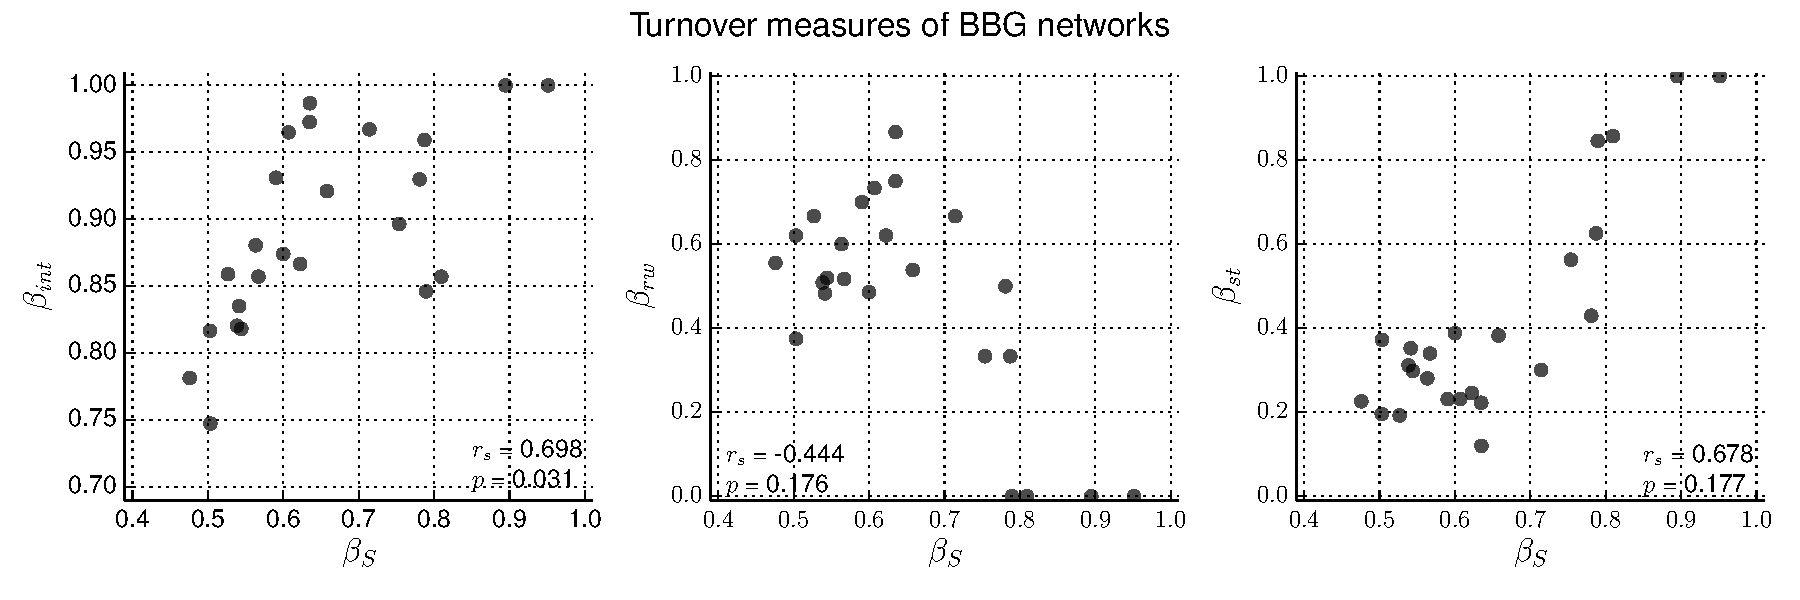
\includegraphics[width=1.1\textwidth]{turnoversbivariate(old).pdf}
    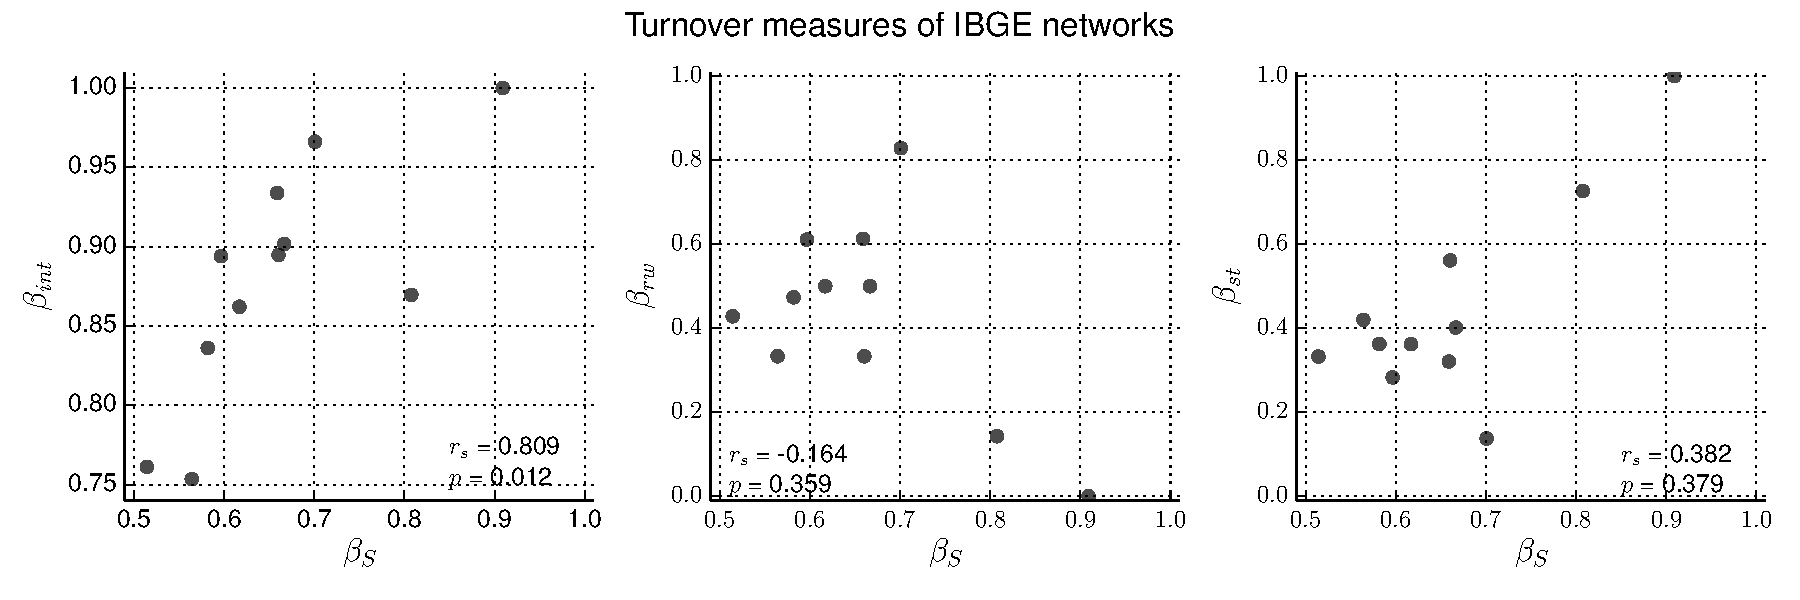
\includegraphics[width=1.1\textwidth]{turnoversbivariate(new).pdf}
     \captionof{figure}{\setstretch{1.3}Trends between species turnover~($\beta_{S}$) and interaction turnover~($\beta_{int}$), interaction rewiring~($\beta_{rw}$) and network dissimilarity due to $\beta_{S}$~($\beta_{st}$). \\   \footnotesize  ( $r_{s}$: Spearman's rank correlation coefficient; p: p-values generated using Monte Carlo simulations.)}
       \label{fig: turnoversbivariate}
\end{figure}
\vspace{2cm}

Surprisingly, $\beta_{st}$ does not associate with $\beta_{S}$ at both sites~(\hyperref[table: turnovers]{Table S\ref{table: turnovers}})(\autoref{fig: turnoversbivariate}). $\beta_{st}$ indirectly reflects the contribution of $\beta_{S}$ to $\beta_{int}$ and will theoretically increase as $\beta_{S}$ increases. However, due to insufficient sampling and climatic conditions, interactions were unequally sampled across time, resulting in inflated $\beta_{rw}$ values~(\autoref{fig: networks}). As $\beta_{st}$ is obtained by subtracting $\beta_{rw}$ from $\beta_{int}$, this results in $\beta_{st}$ values being underestimated and the lack of relationship between $\beta_{st}$ and $\beta_{S}$. Thus, $\beta_{rw}$ and $\beta_{st}$ will hereafter not be used for analysis. Nonetheless, $\beta_{int}$, $\beta_{S}$, $\beta_{Plant}$ and $\beta_{Bee}$ accumulate less error than $\beta_{rw}$ and are more robust to sampling efforts~\citep{Poisot2012}. These measures are hence utilised for further analysis. \\
\\

\begin{figure}[H]
  \centering
    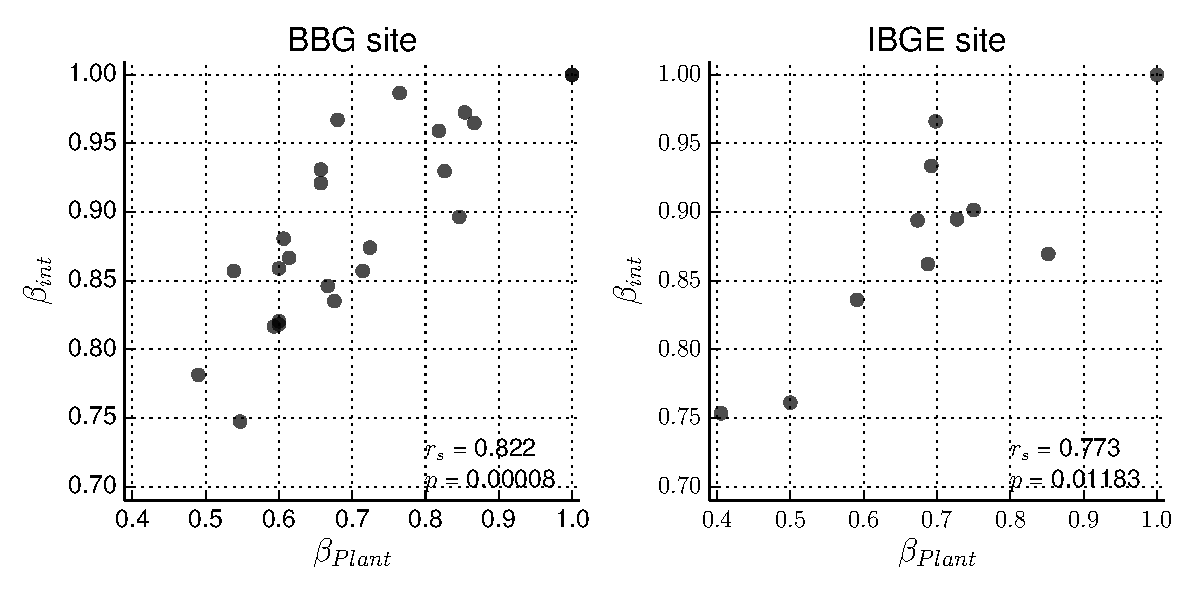
\includegraphics[width=\textwidth]{plantturnover.pdf}
     \captionof{figure}{  \setstretch{1.3} Plant turnover~($\beta_{Plant}$) drives interaction turnover~($\beta_{int}$). \\ \footnotesize
     A high $\beta_{Plant}$ and/or $\beta_{int}$ indicates a high dissimilarity between interactions and/or plant communities of two networks.
     ( $r_{s}$: Spearman's rank correlation coefficient; p: values generated using Monte Carlo simulations.)}
       \label{fig: plantturnover}
\end{figure} 

\subsection{The effect of climatic factors on plant and interaction turnover.}
\label{subsec: climate}
Spearman's correlation coefficients indicate that there exist a seasonal effect on the trends between climatic factors and $\beta_{Plant}$ and $\beta_{int}$~(\hyperref[table: climaticturnover]{Table S\ref{table: climaticturnover}}). Hence, a linear regression model was used to predict $\beta_{Plant}$ using temperature, precipitation, season and their interactions. Temperature difference and precipitation difference between months do not explain $\beta_{Plant}$ as the null model was obtained after minimising the linear regression model (intercept=0.706$\pm$0.0284, p$<$0.0001, df=23, res.s.e.=0.139). \\
\\
\\
By contrast, under the average model, networks experience a lower $\beta_{Plant}$ during the wet season and $\beta_{Plant}$ increases as average temperature increases during the wet season~(adj.r$^{2}$=0.122, F$_{3,20}$=2.07, p=0.137)(\hyperref[table: lm]{Table S\ref{table: lm}}). This indicates that the average model is a better model for $\beta_{Plant}$ than the difference model. Nonetheless, the variation inflation factor (VIF) for variables in this minimal model exceeds the recommended value of 3~\citep{Zuur2010}. $\beta_{Plant}$ was hence fitted against average temperature and precipitation within seasons to reduce multicollinearity. \\
\\
Within the dry season, average temperature and average precipitation levels do not explain $\beta_{Plant}$ as the null model was acquired as the minimal model (intercept=0.700$\pm$0.0447, p$<$0.0001, df=11, res.s.e.=0.155). However, within the wet season, minimal model shows that average temperature explains significant variation in $\beta_{Plant}$ (adj.r$^{2}$=0.504, F$_{1,10}$=12.18, p= 0.00583) and $\beta_{Plant}$ increases as average temperature increases (intercept: -4.57, s.e.=1.51, p=0.0129; slope: 0.239, s.e.=0.0685, p=0.00583). \\
\\
Under both models, the null model was obtained as the minimal model when using temperature, precipitation, season and their interactions to explain $\beta_{int}$ (intercept=0.891$\pm$0.0146, p$<$0.0001, df=23, res.s.e.=0.0714). As expected from previous results, $\beta_{Plant}$ explains significant variation in $\beta_{int}$ (adj.r$^{2}$=0.653, F$_{1,22}$=44.35, p$<$0.0001). $\beta_{Plant}$ increases as $\beta_{int}$ increases (intercept: 0.594, s.e.=0.0453, p$<$0.0001; slope: 0.421, s.e.=0.0631, p$<$0.0001). \\

\newpage
\section{Discussion} % 2118 words
Ecological networks have previously been assumed to be invariant across long time periods, leading to species interactions being largely ignored~\citep{Poisot2015}. However, this study demonstrates, in agreement with previous studies on temporal networks, that dissimilarity between monthly networks is consistently high~\citep{Olesen2008, Burkle2013, CaraDonna2017}. Nonetheless, there are surprisingly no apparent differences between turnover values within seasons and between seasons~(\hyperref[table: turnovers]{Table S\ref{table: turnovers}}, \hyperref[fig: turnovertimeplotold]{Figure \ref{fig: turnovertimeplotold}}, \hyperref[fig: turnovertimeplotnew]{Figure \ref{fig: turnovertimeplotnew}}). \\
\\
Furthermore, this study shows that $\beta_{Plant}$ is a major contributor of $\beta_{int}$ and is a good predictor of $\beta_{int}$~(\hyperref[subsec: turnover]{Results \ref{subsec: turnover}}). In \cite{Alarcon2008}, the Bray-Curtis dissimilarity index and a different approach were utilised to compare species turnover to plant-pollinator interactions in a montane meadow system in California, United States. Unexpectedly, the study has likewise demonstrated that the degree of similarity between flowering plant compositions of two weekly networks mirrors the extent of similarity between the two corresponding interaction networks~\citep{Alarcon2008}. \\
\\
In contrast, \cite{Poisot2015} and \cite{CaraDonna2017} argue that interaction rewiring is indispensable in estimating interaction turnover. \cite{CaraDonna2017} postulates that $\beta_{st}$ only coincides with $\beta_{int}$ when both values are elevated at seasonal transitions. Within seasons, $\beta_{st}$ falls while $\beta_{rw}$ rises~\citep{CaraDonna2017}. Due to inflated $\beta_{st}$ values, the presence of such a trend in the Cerrado datasets cannot be determined. Nonetheless, randomising networks using the Monte Carlo process has illustrated that the strong collinearity between $\beta_{Plant}$ and $\beta_{int}$ did not occur by chance and strengthens the case that $\beta_{Plant}$ is a major driver of $\beta_{int}$~(\hyperref[subsec: turnover]{Results \ref{subsec: turnover}}). \\
\\
To date, to the best of my knowledge, there has been no research investigating the effect of climatic factors on temporal plant-pollinator interaction turnover~\citep{Burkle2011, Scaven2013}. Although it is widely agreed that the climate affects the physiology of plants and in certain cases, even bees, little is known about how or if these responses do influence plant-pollinator interactions~\citep{Hughes2000, Parmesan2003}. Most temporal network studies have focused on how the climate can affect network structure, species richness or abundance and even possible mismatches between plant flowering and insect emergence~\citep{BASILIO2006, Alarcon2008, MartinGonzalez2009, Schweiger2010}. However, although climate change may not have a direct harmful impact on species, it could have a different opposite effect on plant-pollinator interactions~\citep{Hegland2009, Scaven2013}. \\
\\
Plant-pollinator interactions are ecologically significant and economically important. Pollination visits drive plant diversity and maintains plant reproduction and lifecycles~\citep{Olesen2008}. Being at the bottom of the food chain, changes in the stability of plant communities can have rippling effects across entire ecosystems~\citep{Scaven2013}. Moreover, pollination services contribute annually an estimated \$220 billion world-wide to the global economy~\citep{Gallai2009}. Hence, there is an urgent need to study the impact of climate change on interaction networks~\citep{Scaven2013}. \\
\\
To study the impact of climate on turnover measures, two different climate models were used. Average climatic values of two subsequent months proved to be a better explanatory variable of $\beta_{Plant}$ than the use of differences between climatic values of two networks. This further supports the average model with the hypothesis that two networks experiencing the same climate will still yield a positive $\beta_{int}$. This is a logical scenario as networks constantly experience turnover across time even if temperature and all other climatic factors were kept constant~(\hyperref[subsec: climate]{Results \ref{subsec: climate}}).\\
\\
Although both precipitation and temperature do not explain the variation in $\beta_{int}$, $\beta_{int}$ is driven by $\beta_{S}$ and $\beta_{Plant}$. $\beta_{int}$ has a weaker correlation with $\beta_{S}$ as compared to its relationship with $\beta_{Plant}$. This could be due to the non-significant correlation between $\beta_{Bee}$ and $\beta_{Plant}$~(\hyperref[subsec: climate]{Results \ref{subsec: climate}}), indicating that different factors drive the turnover of the two different species. \\
\\
Indeed, plants, and especially flowers, are more sensitive to climatic changes than bees. Plants living under higher temperatures have been shown to produce fewer flowers as temperature elevates, resulting in a higher $\beta_{Plant}$~\citep{Scaven2013}, hence explaining the positive correlation between $\beta_{Plant}$ and temperature during the wet season~(\hyperref[subsec: climate]{Results \ref{subsec: climate}}). Nevertheless, this is surprising as the range of temperatures of the BBG dataset is less than 5$\degree$C~(\hyperref[fig: climatetimeplotold]{Figure \ref{fig: climatetimeplotold}}), and thus further illustrates the extent of sensitivity of plants to the climate. In the Cerrado, dry season flowering is restricted in species with shallow root systems~\citep{Oliveira2002, Gottsberger2006} and therefore, flowering plants may not respond to temperature changes during the dry season as no flowering has occurred, accounting for the lack of an association between $\beta_{Plant}$ and temperature during this season. Although $\beta_{int}$ is consistently high throughout the year, there appears to be a seasonal difference in factors that drive turnover~(\hyperref[subsec: turnover]{Results \ref{subsec: turnover}}).\\
\\
Unexpectedly, despite the drastic difference between the precipitation level of dry and wet seasons, precipitation was an insignificant factor in explaining $\beta_{Plant}$~(\hyperref[subsec: climate]{Results \ref{subsec: climate}}). Plants in the Cerrado have evolved mechanisms to survive cycles of extreme drought and may therefore be less sensitive to changes in precipitation~\citep{Oliveira2002, Gottsberger2006}. Nonetheless, precipitation may account for the seasonal effect that temperature has on $\beta_{Plant}$, but more complex models and data will be required to support this hypothesis. \\
\\
Lastly, $\beta_{Plant}$ drives $\beta_{S}$ at the IBGE site but not at the BBG site~(\hyperref[subsec: turnover]{Results \ref{subsec: turnover}}). The IBGE survey site is covered with sparse distribution of plants, consisting mainly of grasses and shrubs. In contrast, the BBG community comprises of mainly large shrubs, lianas and trees which have a longer lifespan~\citep{Eiten1972}, and hence, BBG communities may experience a lower $\beta_{Plant}$ than IBGE communities. The higher $\beta_{Plant}$ of the IBGE communities may hence contribute to $\beta_{S}$ to a larger extent, resulting in a positive correlation. Further analysis is required to explore this relationship. However, due to time constraints, this line of investigation was not pursued. 

\subsection{Limitations}

$\beta_{int}$ in the Cerrado was higher than previously reported week-to-week and year-to-year $\beta_{int}$ values~\citep{CaraDonna2017}(\hyperref[table: turnovers]{Table S\ref{table: turnovers}}). In \cite{CaraDonna2017}, sampling only took place during the flowering period as the area is mostly covered by snow for the rest of the year. $\beta_{int}$ values could therefore be relatively lower due to climatic factors remaining relatively similar throughout the flowering season in the temperate region. As plants can only be pollinated during the three short months annually, temperate plant communities have a longer mean flowering time than those in the tropics~\citep{Bawa1990}, resulting in a lower $\beta_{Plant}$. Lower $\beta_{Plant}$ values could thereafter lead to lower $\beta_{int}$ values. However, as no month-to-month $\beta_{int}$ or $\beta_{Plant}$ values were made available, no direct comparison of $\beta$-diversity between temperate and tropic regions can be made~\citep{CaraDonna2017}. \\
\\
Moreover, other studies of temporal plant-pollinator networks utilises one of the other 23 $\beta$-diversity measures, making it highly difficult for any direct comparisons~\citep{BASILIO2006, Alarcon2008, Olesen2008, Burkle2013}. Little consensus has yet been reached as to which $\beta$-dissimilarity measure best reflects temporal and spatial $\beta$-diversity, resulting in a large number of different approaches and contradictory results~\citep{Koleff2003, Poisot2015}.\\
\\
Insufficient sampling is yet another problem, which can lead to inflated $\beta_{rw}$ values, as networks falsely appear to be more dissimilar than in reality due to missing interactions~\citep{Vazquez2007, Dormann2009, Poisot2012a}. This problem is sometimes unavoidable due to existing weather conditions and can be illustrated by the abnormally high $\beta_{st}$ and $\beta_{int}$ between the months of November 1995 to January 1996 at the BBG site~(\hyperref[table: turnovers]{Table S\ref{table: turnovers}}, \hyperref[fig: turnovertimeplotold]{Figure \ref{fig: turnovertimeplotold}}). Removing these data points would have significantly reduced the sample size of the BBG dataset. As $\beta_{int}$, $\beta_{S}$, $\beta_{plant}$ and $\beta_{bee}$ are more robust to sampling error, these data points were included and tests which are robust to outliers, such as the Spearman correlation coefficient test was used. Monte Carlo simulation was thereafter carried out to reduce sampling bias.\\
\\
8.19\% and 4.61\% of all unique interactions appeared in three or more monthly networks at the BBG and IBGE sites respectively~(\autoref{fig: networks}). Although this may have been in part due to insufficient sampling efforts, another plausible cause is the high biodiversity levels found in the tropics. 45 flowering plants and 74 pollinators were observed over 3 years of study in ~\cite{CaraDonna2017}. Comparatively, within the 12-month study period at IBGE, 111 species of bees and 93 species of plants were already recorded~(\hyperref[sec: results]{Section \ref{sec: results}}) and yet it is apparent that there exist many missing interactions. $\beta_{int}$ values may hence be higher in the tropics than in the temperate regions due to the species richness found in the tropical biome. Due to the lack of temporal network data in the tropics, there is no support for this hypothesis yet.

\subsection{Conclusion and Future Research}
Understanding temporal interaction networks is crucial in the conservation of ecosystems as protecting or restoring an ecosystem requires approaches that restores its interaction and functions for its long term stability. Climate change has already influenced plant phenology, resulting in plants blooming earlier than ever before~\citep{Cleland2007,Miller-Rushing2008}. Hence, there is an urgent need to investigate and validate the drivers of dissimilarity of temporal networks, in order to understand the extent to which climate and plant phenology can affect species interaction. A decrease in pollination visits globally will result in decreased plant diversity and stability of plant communities. In return, this will adversely affect our ecosystems and food security~\citep{Schweiger2010, Burkle2011}. \\
\\
Nonetheless, correlation of variables does not relate to causation. Experimental approaches are therefore required to test out these predictions on small artificially manipulated ecosystems. If the spatial and temporal scale of experiments are not large enough to significantly affect network turnover, available datasets across diverse habitats with varying climates can be compared to support these predictions~\citep{Burkle2009, Burkle2011}. In fact, spatial network studies which utilises national gradients of climatic factors have already provided several insights. In the West Indies, plant species become increasingly specialised with elevated precipitation levels and decreased temperatures~\citep{MartinGonzalez2009}. Hence, research on spatial networks are necessary to further support the predictions found in studies of temporal interaction networks.\\
\\
Moreover, before further progress can be made in this field of study, it is crucial to establish a definition and measure of $\beta$-diversity that most researchers can come to a consensus to. Alternatively, future research should either utilise more than one measure of $\beta$-diversity, publish their original datasets or release the a, b and c values commonly used for most $\beta$-dissimilarity measures. This will enable comparison of results across different datasets and reveal more insights into characteristics of interaction turnover. Collecting temporal network data is time-consuming and require large amounts of sampling to prevent inflated values of network dissimilarity~\citep{Koleff2003, Burkle2011, Poisot2015}. Hence, compiling available data and comparing networks in both the temperate and tropical regions will be necessary to paint a clearer picture of interaction networks. \\
\\
With better $\beta$-diversity measures, drivers of temporal interaction turnover can be better understood. For example, sensitivity of interactions to the climate, predictors of interaction turnover and the significance of phenology in interaction networks are fascinating and essential topics in which we currently lack an understanding of~\citep{Poisot2012}. Furthermore, current datasets of temporal networks are sorely lacking in both resolution and length of study. Currently, the best dataset available originates from a four year study of a Phryganic community in Greece~\citep{Petanidou1991}. 
Additional long-term studies across different ecosystems are crucial to further our understanding of the temporal variability of interactions~\citep{Burkle2011}.\\
\\
In conclusion, this study presents evidence that month-to-month interaction networks are highly dissimilar from each other and is the first of its kind to study temporal networks in the Cerrado as well as to directly link climatic changes to temporal plant turnover, and thereafter temporal interaction turnover. Future studies on temporal networks of finer resolutions will be able to greatly improve our understanding of interaction networks and allow us to better protect ecosystems in the face of climate change.

% acknowledgement page
\newpage 
\vspace*{\fill}

{\huge\bfseries Acknowledgements} \label{sec: acknowledgements} \\
\\
\\
\large{I would like to thank Dr. Samraat Pawar for his supervision and guidance throughout this project, as well as  all of my friends who have helped me in one way or another with Python programming. Finally, I would like to thank M. C. Boaventura and S. C. Cappellari for making their datasets available. Field data collection at IBGE was made possible with the support of P. H. Pinheiro, the staff of Reserva Ecol\'{o}gica do IBGE and the graduate program in Ecology at the University of Brasilia. The following experts contributed towards the identification of plants: M. A. da Silva, M. C. Mamede, C. Proen\c{c}a, A. L. Prado, S. L. Silva, L. P. Queiroz, A. Krapovikas, L. F. Oliveira, T. B. Cavalcante, K. Calago, A. E. Ramos, C. Munhoz, F. Silva, M. G. N\'{o}brega, R. C. Martins, and R. C. Oliveira, and the following experts for bee identifications: A. J. C. Aguiar, A. Raw, M. C. Boaventura, G. A. R. Melo, F. Vivallo, and D. Urban.}
\vfill

\newpage
\bibliography{buzz2}
\bibliographystyle{cell}

\newpage
\section{Supplementary Figures}
%%%%%%%%%% Merge with supplemental materials %%%%%%%%%%
%%%%%%%%%% Prefix a "S" to all equations, figures, tables and reset the counter %%%%%%%%%%
\setcounter{equation}{0}
\setcounter{figure}{0}
\setcounter{table}{0}
\makeatletter
\renewcommand{\theequation}{S\arabic{equation}}
\renewcommand{\thefigure}{S\arabic{figure}}
\renewcommand{\bibnumfmt}[1]{[S#1]}
\renewcommand{\citenumfont}[1]{S#1}
%%%%%%%%%% Prefix a "S" to all equations, figures, tables and reset the counter %%%%%%%%%%

%%%%%%%%%%%%%%%%%%%%%%%%%%%%%%%%%%%%

\begin{table}[h]
\centering
\captionof{figure}{\setstretch{1.3}Example of calculating turnover measures of the networks of April and May 2009. \footnotesize Each number represents a bee or plant species and is represented by a node in \autoref{fig: networks} and \hyperref[fig: seasonalnetworks]{Figure \ref{fig: seasonalnetworks}}. Unique interactions of both networks are shown here. Boxes are color coded to show bee and plant species common to both networks.}
\label{fig: calculationex}
\begin{tabular}{|l|l|lll}
\hhline{--~--}
\multicolumn{2}{|l|}{\cellcolor[HTML]{EFEFEF}April 2009} & \multicolumn{1}{l|}{} & \multicolumn{2}{l|}{\cellcolor[HTML]{EFEFEF}May 2009} \\ \hhline{--~--}
\cellcolor[HTML]{EFEFEF}Bee & \cellcolor[HTML]{EFEFEF}Plant & \multicolumn{1}{l|}{} & \multicolumn{1}{l|}{\cellcolor[HTML]{EFEFEF}Bee} & \multicolumn{1}{l|}{\cellcolor[HTML]{EFEFEF}Plant} \\ \hhline{--~--}
\cellcolor[HTML]{E3E5F9}6 & 132 & \multicolumn{1}{l|}{} & \multicolumn{1}{l|}{49} & \multicolumn{1}{l|}{\cellcolor[HTML]{DDF4DC}147} \\ \hhline{--~--}
\cellcolor[HTML]{E3E5F9}22 & 132 & \multicolumn{1}{l|}{} & \multicolumn{1}{l|}{65} & \multicolumn{1}{l|}{\cellcolor[HTML]{DDF4DC}147} \\ \hhline{--~--}
32 & 148 & \multicolumn{1}{l|}{} & \multicolumn{1}{l|}{109} & \multicolumn{1}{l|}{178} \\ \hhline{--~--}
\cellcolor[HTML]{E3E5F9}90 & 155 & \multicolumn{1}{l|}{} & \multicolumn{1}{l|}{\cellcolor[HTML]{E3E5F9}91} & \multicolumn{1}{l|}{\cellcolor[HTML]{DDF4DC}185} \\ \hhline{--~--}
72 & 164 & \multicolumn{1}{l|}{} & \multicolumn{1}{l|}{28} & \multicolumn{1}{l|}{117} \\ \hhline{--~--} 
57 & 166 & \multicolumn{1}{l|}{} & \multicolumn{1}{l|}{16} & \multicolumn{1}{l|}{159} \\ \hhline{--~--} 
57 & \cellcolor[HTML]{DDF4DC}168 & \multicolumn{1}{l|}{} & \multicolumn{1}{l|}{\cellcolor[HTML]{E3E5F9}22} & \multicolumn{1}{l|}{169} \\ \hhline{--~--}
71 & \cellcolor[HTML]{DDF4DC}168 & \multicolumn{1}{l|}{} & \multicolumn{1}{l|}{\cellcolor[HTML]{E3E5F9}90} & \multicolumn{1}{l|}{\cellcolor[HTML]{DDF4DC}185} \\ \hhline{--~--}
\cellcolor[HTML]{E3E5F9}84 & \cellcolor[HTML]{DDF4DC}168 & \multicolumn{1}{l|}{} & \multicolumn{1}{l|}{\cellcolor[HTML]{E3E5F9}17} & \multicolumn{1}{l|}{159} \\ \hhline{--~--}
\cellcolor[HTML]{E3E5F9}91 & 205 & \multicolumn{1}{l|}{} & \multicolumn{1}{l|}{\cellcolor[HTML]{E3E5F9}90} & \multicolumn{1}{l|}{159} \\ \hhline{--~--}
102 & 205 & \multicolumn{1}{l|}{} & \multicolumn{1}{l|}{\cellcolor[HTML]{E3E5F9}6} & \multicolumn{1}{l|}{165} \\ \hhline{--~--} 
\cellcolor[HTML]{E3E5F9}91 & \cellcolor[HTML]{DDF4DC}147 & \multicolumn{1}{l|}{} & \multicolumn{1}{l|}{106} & \multicolumn{1}{l|}{201} \\ \hhline{--~--}
41 & 138 & \multicolumn{1}{l|}{} & \multicolumn{1}{l|}{\cellcolor[HTML]{E3E5F9}90} & \multicolumn{1}{l|}{117} \\ \hhline{--~--}
\cellcolor[HTML]{E3E5F9}17 & 138 & \multicolumn{1}{l|}{} & \multicolumn{1}{l|}{\cellcolor[HTML]{E3E5F9}90} & \multicolumn{1}{l|}{139} \\ \hhline{--~--}
\cellcolor[HTML]{E3E5F9}91 & 164 & \multicolumn{1}{l|}{} & \multicolumn{1}{l|}{70} & \multicolumn{1}{l|}{159} \\ \hhline{--~--} 
9 & 166 & \multicolumn{1}{l|}{} & \multicolumn{1}{l|}{37} & \multicolumn{1}{l|}{161} \\ \hhline{--~--} 
13 & 166 & \multicolumn{1}{l|}{} & \multicolumn{1}{l|}{\cellcolor[HTML]{E3E5F9}84} & \multicolumn{1}{l|}{\cellcolor[HTML]{DDF4DC}168} \\ \hhline{--~--}
76 & 166 &  &  &  \\ \hhline{--~~~}
\cellcolor[HTML]{E3E5F9}91 & \cellcolor[HTML]{DDF4DC}185 &  &  &  \\ \hhline{--~~~}
101 & \cellcolor[HTML]{DDF4DC}185 &  &  &  \\ \hhline{--~~~}
30 & 118 &  &  &  \\ \hhline{--~~~}
\end{tabular}
\end{table}
\vspace{-1.5cm}
%fix numbers

\begin{align*}
	& \textnormal{Whittaker's dissimilarity measure: } & \beta_{W} & = \frac{a + b + c}{(2a + b + c)/2} - 1 \\
	 &\textnormal{Interaction turnover: } & \beta_{int} & = \frac{2 + 19 + 15}{(2*(2) + 19 + 15)/2} - 1 & = 0.895\\
	 &\textnormal{Interaction rewiring: } & \beta_{rw} & = \frac{2 + 1 + 1}{(2*(2) + 1 + 1)/2} - 1 & = 0.333\\
	 &\textnormal{Dissimilarity of interactions due to $\beta_{S}$: } & \beta_{st} & = 0.89474 - 0.33333 & = 0.561 \\
	 \\
	 &\textnormal{Species turnover: } & \beta_{S} & = \frac{9 + 19 + 16}{(2*(9) + 19 + 16)/2} - 1 & = 0.660\\
	 &\textnormal{Bee turnover: } & \beta_{Bee} & = \frac{6 + 11 + 8}{(2*(6) + 11 + 8)/2} - 1 & = 0.613\\
	 &\textnormal{Plant turnover: } & \beta_{Plant} & = \frac{3 + 8 + 8}{(2*(3) + 8 + 8)/2} - 1 & = 0.727\\
\end{align*}
%%%%%%%%%%%%%%%%%%%%%%%%%%%%%%%%%%%%
%%%%%%%%%%%%%%%%%%%%%%%%%%%%%%%%%%%%

\newpage
\begin{landscape}

\vspace*{\fill}
\begin{figure}[H]
  \centering
    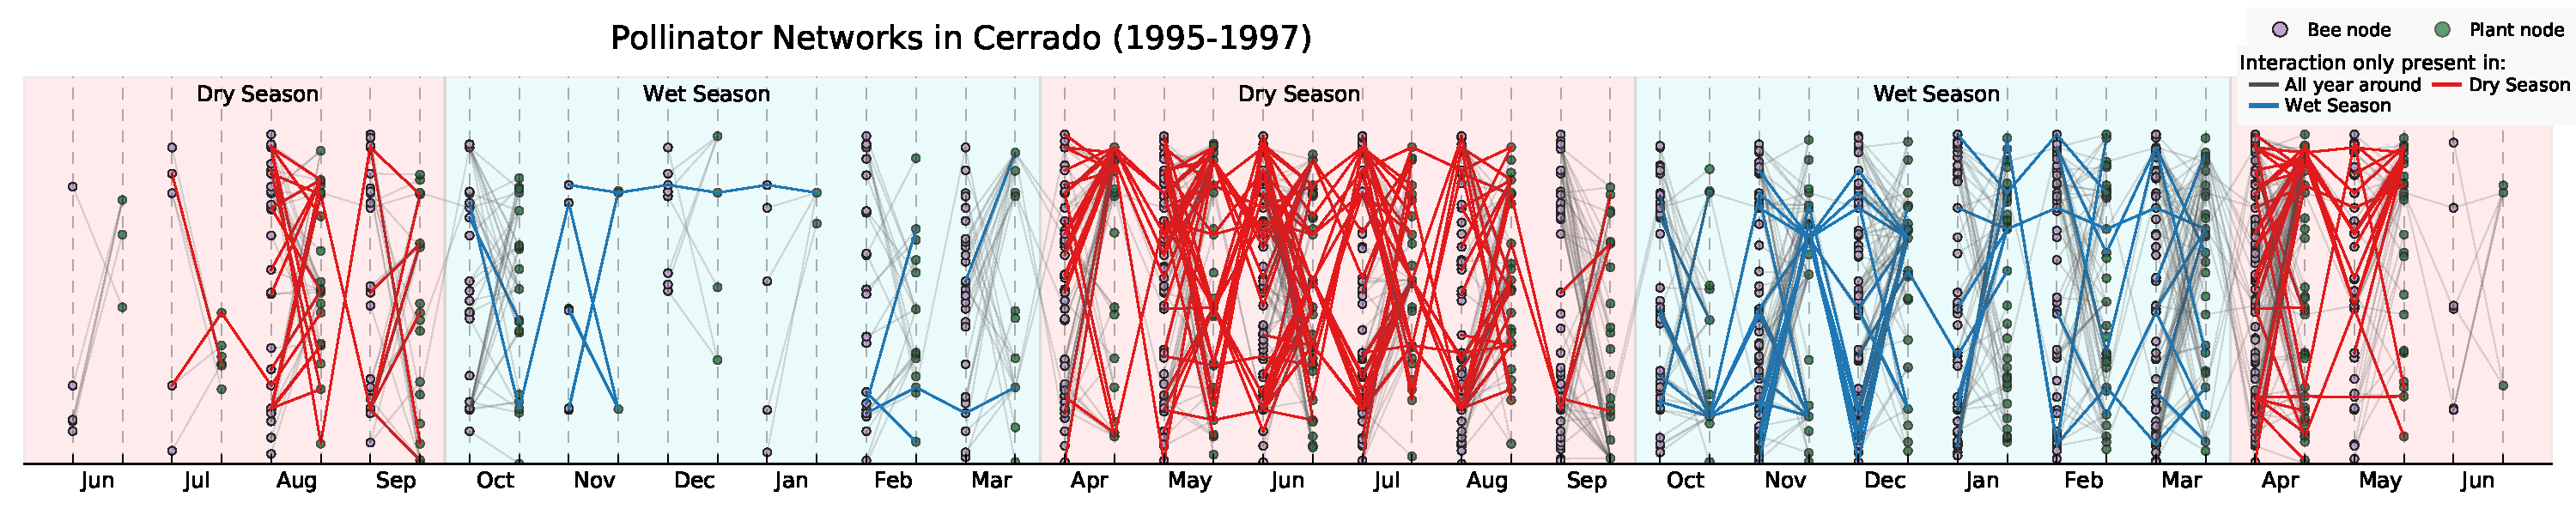
\includegraphics[width=260mm]{seasonalnetwork(old).pdf} \\
    \vspace{1cm}
    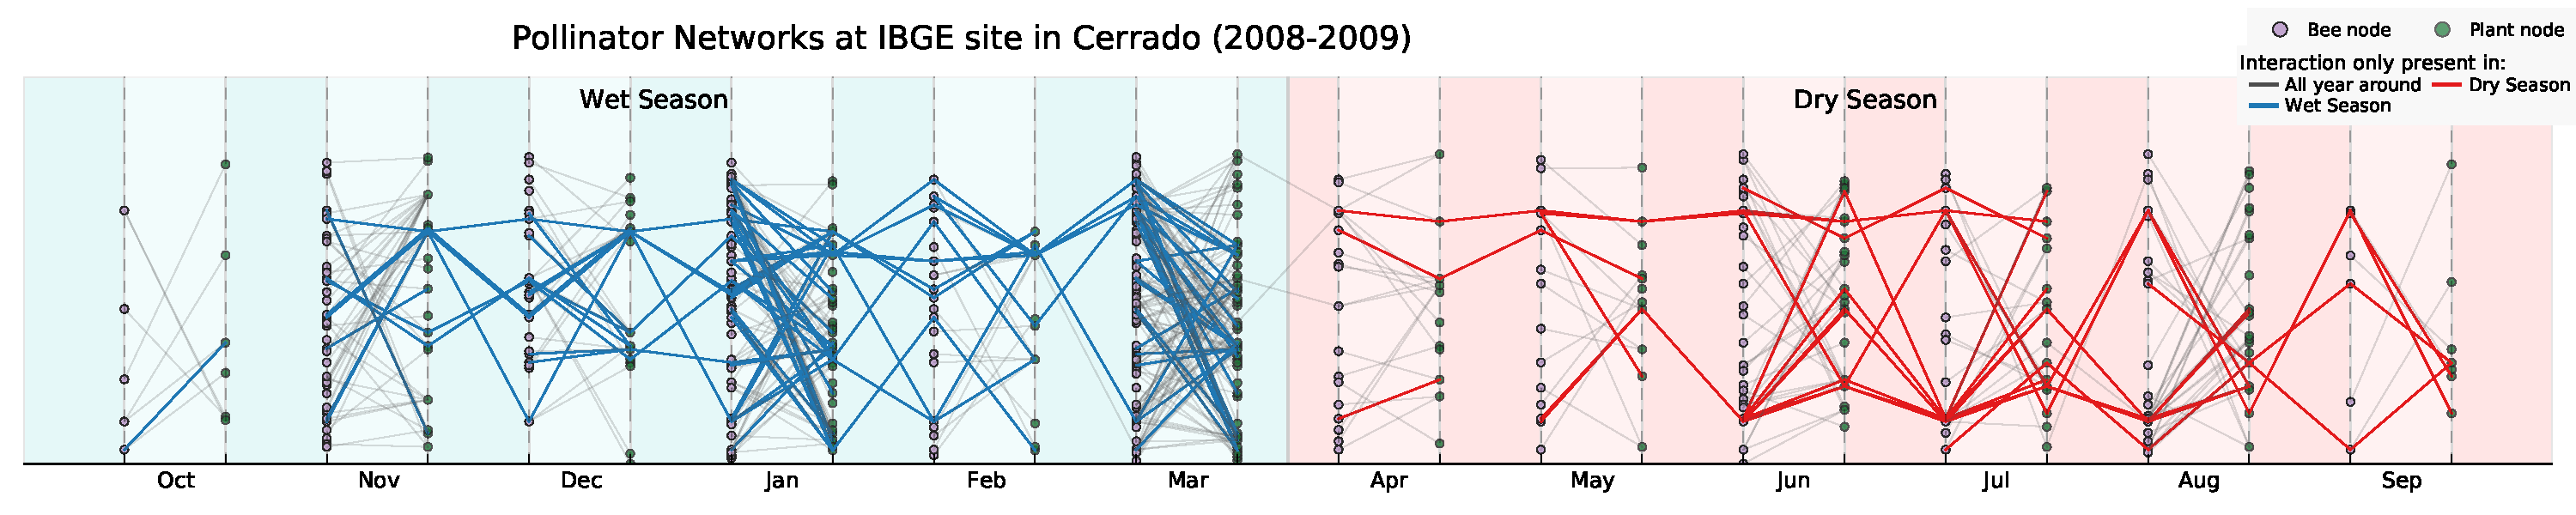
\includegraphics[width=260mm]{seasonalnetwork(new).pdf}
    \captionof{figure}{\setstretch{1.3} \setstretch{1.3} Monthly bee pollinator networks from Jun 1995 to Jun 1997 (BBG site) and from Oct 2008 to Sep 2009 (IBGE site).\\ \footnotesize Every node in a monthly network represents a distinct plant or bee species. Each link between plant and bee nodes represent a unique pollination visit in the corresponding month. Links between monthly networks show interactions recorded in both monthly networks. Background of plot is colour-coded to reflect the seasons: blue - wet season; red - dry season. Each link is colour-coded to reflect its period of activity: blue ? only present during the wet season; red ? only present during the dry season; black ? present in both seasons.}
    \label{fig: seasonalnetworks}
\end{figure}
	\vspace*{\fill}

\begin{figure}[H]
  \centering
    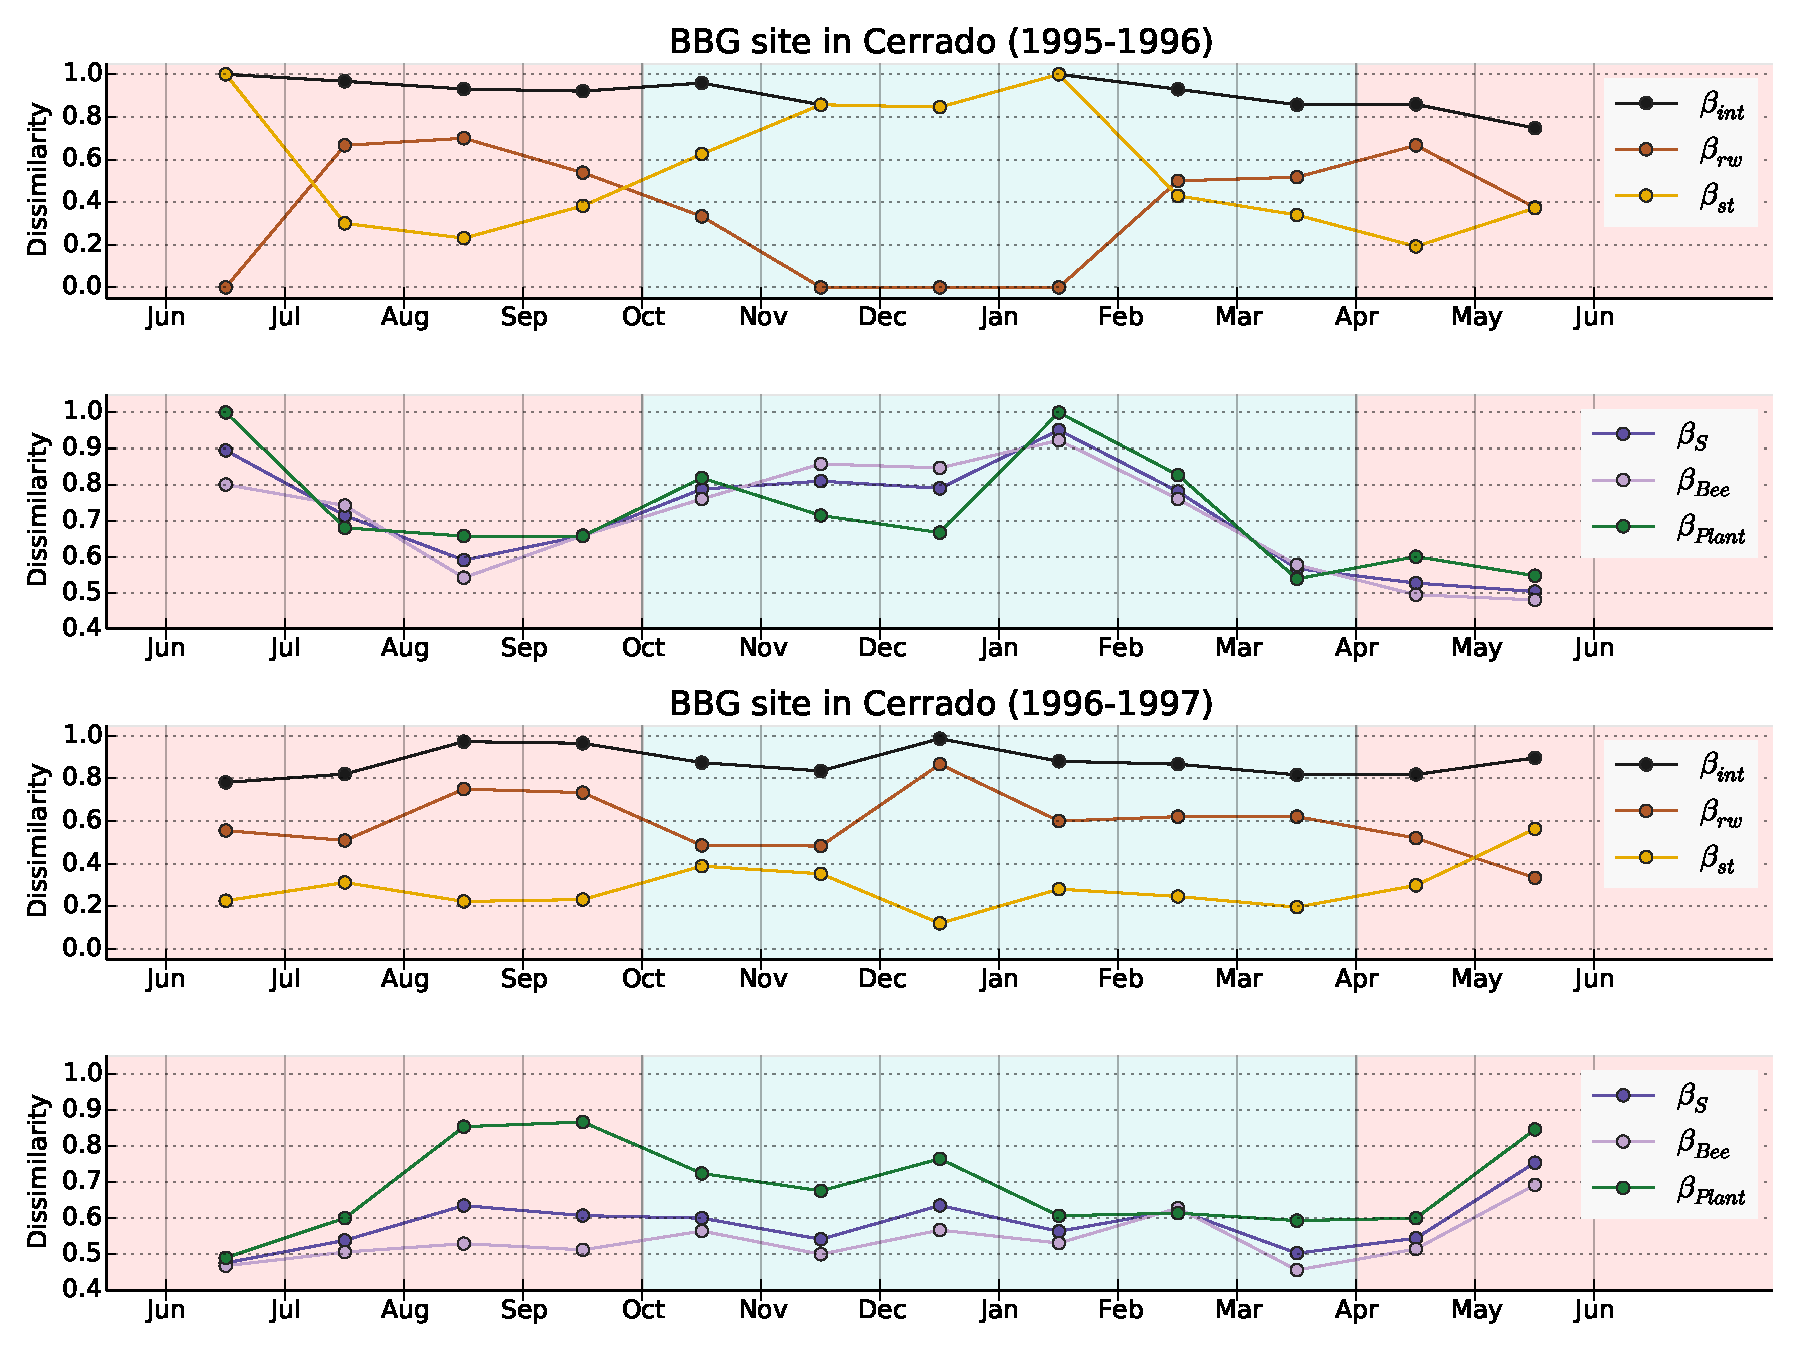
\includegraphics[width=200mm]{TimeplotTurnovers(old).pdf} \\
    \captionof{figure}{\setstretch{1.3} Time series plot of turnover measures from Jun 1995 to Jun 1997 (BBG site).}
    \label{fig: turnovertimeplotold}
\end{figure}

\begin{figure}[H]
  \centering
    \includegraphics[width=200mm]{Climate(old).pdf} \\
    \captionof{figure}{\setstretch{1.3} Time series plot of climatic factors from Jun 1995 to Jun 1997 (BBG site). \\ \footnotesize
    (Average model: average of precipitation/temperature of two subsequent months; Difference model: difference between precipitation/temperature of two subsequent months)}
    \label{fig: climatetimeplotold}
\end{figure}

\begin{figure}[H]
  \centering
    \includegraphics[width=180mm, height = 65mm]{TimeplotTurnovers(New).pdf} \\
    \captionof{figure}{\setstretch{1.3} Time series plot of turnover measures from Oct 2008 to Sep 2009 (IBGE site).}
    \label{fig: turnovertimeplotnew}
\end{figure}

\begin{figure}[H]
  \centering
    \includegraphics[width=185mm, height = 65mm]{Climate(new).pdf} \\
    \captionof{figure}{Time series plot of climatic factors from Oct 2008 to Sep 2009 (IBGE site). \\ \footnotesize
    (Average model: average of precipitation/temperature of two subsequent months; Difference model: difference between precipitation/temperature of two subsequent months)}
    \label{fig: climatetimeplotnew}
\end{figure}

\end{landscape}

%%%%%%%%%%%%%%%%%%%%%%%%%%%%%%%%%%%%
%%%%%%%%%%%%%%%%%%%%%%%%%%%%%%%%%%%%%%%%%%%%%%
\begin{table}[h]
\centering
\setstretch{1.3}
\captionof{table}{Month-to-month turnover values for all dissimilarity measures at both the Bras\'ilia's Botanical Garden Protected Area (BBG) and Reserva Ecol\'ogica do IBGE (IBGE) sites.}
\label{table: turnovers}
\resizebox{\textwidth}{!}{%
\begin{tabular}{|c|c|r|r|r|r|r|r|r|r|c|}
\hline
\rowcolor[HTML]{EFEFEF} 
Year & Months  & \multicolumn{1}{c|}{$\beta_{int}$}   & \multicolumn{1}{c|}{$\beta_{rw}$}    & \multicolumn{1}{c|}{$\beta_{st}$}    &\multicolumn{1}{c|}{$\beta_{rw}$/$\beta_{int}$}  & \multicolumn{1}{c|}{$\beta_{st}$/$\beta_{int}$}  &  \multicolumn{1}{c|}{$\beta_{S}$}     &  \multicolumn{1}{c|}{$\beta_{Bee}$} &  \multicolumn{1}{c|}{$\beta_{Plant}$}    & Site \\ \hline
1995 & Jun-Jul & 1     & 0     & 1     & 0      & 1      & 0.895 & 0.8   & 1     & BBG  \\ \hline
1995 & Jul-Aug & 0.967 & 0.667 & 0.301 & 0.689  & 0.311  & 0.714 & 0.742 & 0.68  & BBG  \\ \hline
1995 & Aug-Sep & 0.931 & 0.7   & 0.231 & 0.752  & 0.248  & 0.59  & 0.542 & 0.657 & BBG  \\ \hline
1995 & Sep-Oct & 0.921 & 0.538 & 0.383 & 0.585  & 0.415  & 0.658 & 0.659 & 0.657 & BBG  \\ \hline
1995 & Oct-Nov & 0.959 & 0.333 & 0.626 & 0.348  & 0.652  & 0.787 & 0.76  & 0.818 & BBG  \\ \hline
1995 & Nov-Dec & 0.857 & 0     & 0.857 & 0      & 1      & 0.81  & 0.857 & 0.714 & BBG  \\ \hline
1995 & Dec-Jan & 0.846 & 0     & 0.846 & 0      & 1      & 0.789 & 0.846 & 0.667 & BBG  \\ \hline
1996 & Jan-Feb & 1     & 0     & 1     & 0      & 1      & 0.951 & 0.923 & 1     & BBG  \\ \hline
1996 & Feb-Mar & 0.93  & 0.5   & 0.43  & 0.538  & 0.462  & 0.781 & 0.76  & 0.826 & BBG  \\ \hline
1996 & Mar-Apr & 0.857 & 0.517 & 0.34  & 0.603  & 0.397  & 0.567 & 0.577 & 0.538 & BBG  \\ \hline
1996 & Apr-May & 0.859 & 0.667 & 0.192 & 0.776  & 0.224  & 0.527 & 0.495 & 0.6   & BBG  \\ \hline
1996 & May-Jun & 0.747 & 0.375 & 0.372 & 0.502  & 0.498  & 0.503 & 0.48  & 0.547 & BBG  \\ \hline
1996 & Jun-Jul & 0.781 & 0.556 & 0.226 & 0.711  & 0.289  & 0.476 & 0.468 & 0.49  & BBG  \\ \hline
1996 & Jul-Aug & 0.821 & 0.509 & 0.312 & 0.62   & 0.38   & 0.538 & 0.506 & 0.6   & BBG  \\ \hline
1996 & Aug-Sep & 0.973 & 0.75  & 0.223 & 0.771  & 0.229  & 0.635 & 0.529 & 0.854 & BBG  \\ \hline
1996 & Sep-Oct & 0.965 & 0.733 & 0.232 & 0.76   & 0.24   & 0.607 & 0.512 & 0.867 & BBG  \\ \hline
1996 & Oct-Nov & 0.874 & 0.486 & 0.388 & 0.556  & 0.444  & 0.6   & 0.564 & 0.724 & BBG  \\ \hline
1996 & Nov-Dec & 0.835 & 0.483 & 0.352 & 0.578  & 0.422  & 0.541 & 0.5   & 0.676 & BBG  \\ \hline
1996 & Dec-Jan & 0.987 & 0.867 & 0.12  & 0.878  & 0.122  & 0.635 & 0.567 & 0.765 & BBG  \\ \hline
1997 & Jan-Feb & 0.881 & 0.6   & 0.281 & 0.681  & 0.319  & 0.563 & 0.531 & 0.607 & BBG  \\ \hline
1997 & Feb-Mar & 0.867 & 0.621 & 0.246 & 0.716  & 0.284  & 0.622 & 0.628 & 0.614 & BBG  \\ \hline
1997 & Mar-Apr & 0.817 & 0.621 & 0.196 & 0.76   & 0.24   & 0.503 & 0.456 & 0.593 & BBG  \\ \hline
1997 & Apr-May & 0.818 & 0.52  & 0.298 & 0.636  & 0.364  & 0.544 & 0.515 & 0.6   & BBG  \\ \hline
1997 & May-Jun & 0.897 & 0.333 & 0.563 & 0.372  & 0.628  & 0.754 & 0.692 & 0.846 & BBG  \\ \hline
2008 & Oct-Nov & 1     & 0     & 1     & 0      & 1      & 0.909 & 0.86  & 1     & IBGE \\ \hline
2008 & Nov-Dec & 0.862 & 0.5   & 0.362 & 0.58   & 0.42   & 0.617 & 0.581 & 0.688 & IBGE \\ \hline
2008 & Dec-Jan & 0.894 & 0.611 & 0.283 & 0.684  & 0.316  & 0.597 & 0.543 & 0.673 & IBGE \\ \hline
2009 & Jan-Feb & 0.836 & 0.474 & 0.362 & 0.567  & 0.433  & 0.582 & 0.576 & 0.591 & IBGE \\ \hline
2009 & Feb-Mar & 0.934 & 0.613 & 0.321 & 0.656  & 0.344  & 0.659 & 0.636 & 0.692 & IBGE \\ \hline
2009 & Mar-Apr & 0.966 & 0.829 & 0.138 & 0.858  & 0.142  & 0.701 & 0.703 & 0.698 & IBGE \\ \hline
2009 & Apr-May & 0.895 & 0.333 & 0.561 & 0.373  & 0.627  & 0.660  & 0.613 & 0.727 & IBGE \\ \hline
2009 & May-Jun & 0.902 & 0.5   & 0.402 & 0.555  & 0.445  & 0.667 & 0.6   & 0.75  & IBGE \\ \hline
2009 & Jun-Jul & 0.753 & 0.333 & 0.42  & 0.442  & 0.558  & 0.564 & 0.707 & 0.405 & IBGE \\ \hline
2009 & Jul-Aug & 0.761 & 0.429 & 0.333 & 0.563  & 0.437  & 0.514 & 0.529 & 0.5   & IBGE \\ \hline
2009 & Aug-Sep & 0.87  & 0.143 & 0.727 & 0.164  & 0.836  & 0.808 & 0.76  & 0.852 & IBGE \\ \hline
\end{tabular}%
}
\end{table}

%%%%%%%%%%%%%%%%%%%%%%%%%%%%%%%%%%%%%%%%%%%%%%
%%%%%%%%%%%%%%%%%%%%%%%%%%%%%%%%%%%%%%%%%%%%%%

\begin{table}[]
\centering
\setstretch{1.3}
\captionof{table}{Climate information obtained from IBGE's weather station. \\
\footnotesize Daily average temperature was calculated using the minimum and maximum temperature of each day. The median value of daily temperatures was then obtained for each month and used for data analysis. Precipitation values were acquired by adding together total amount of rainfall that occurred throughout the month.}
\label{table: climate}
\resizebox{0.6\textwidth}{!}{%
\begin{tabular}{|r|c|r|r|}
\hline
\rowcolor[HTML]{EFEFEF} 
Year & Month & Precipitation / mm & Temperature / \degree C \\ \hline
1995 & Jun & 0 & 18.7 \\ \hline
1995 & Jul & 0 & 19.4 \\ \hline
1995 & Aug & 0 & 20.9 \\ \hline
1995 & Sep & 5 & 22.4 \\ \hline
1995 & Oct & 86.5 & 23.5 \\ \hline
1995 & Nov & 292.1 & 21.6 \\ \hline
1995 & Dec & 328.3 & 21.9 \\ \hline
1996 & Jan & 66 & 22.3 \\ \hline
1996 & Feb & 190 & 22.3 \\ \hline
1996 & Mar & 304.7 & 22.4 \\ \hline
1996 & Apr & 39.7 & 21.2 \\ \hline
1996 & May & 26.5 & 20.4 \\ \hline
1996 & Jun & 0 & 18.4 \\ \hline
1996 & Jul & 0 & 18.7 \\ \hline
1996 & Aug & 48 & 20.4 \\ \hline
1996 & Sep & 37.6 & 22.4 \\ \hline
1996 & Oct & 116.3 & 23 \\ \hline
1996 & Nov & 261.2 & 22.1 \\ \hline
1996 & Dec & 293.6 & 22.7 \\ \hline
1997 & Jan & 358 & 21.7 \\ \hline
1997 & Feb & 104.3 & 22.1 \\ \hline
1997 & Mar & 304.2 & 21.6 \\ \hline
1997 & Apr & 148.1 & 21.2 \\ \hline
1997 & May & 114.2 & 19 \\ \hline
1997 & Jun & 21.4 & 18.8 \\ \hline
2008 & Oct & 29.8 & 24 \\ \hline
2008 & Nov & 196.9 & 22.2 \\ \hline
2008 & Dec & 270.6 & 22.1 \\ \hline
2009 & Jan & 179.8 & 22.3 \\ \hline
2009 & Feb & 153.3 & 22.1 \\ \hline
2009 & Mar & 171.7 & 22.2 \\ \hline
2009 & Apr & 225.2 & 21.3 \\ \hline
2009 & May & 43.3 & 19.4 \\ \hline
2009 & Jun & 26.2 & 18 \\ \hline
2009 & Jul & 0 & 19 \\ \hline
2009 & Aug & 31.9 & 19.8 \\ \hline
2009 & Sep & 36.2 & 22.9 \\ \hline
\end{tabular}%
}
\end{table}

%%%%%%%%%%%%%%%%%%%%%%%%%%%%%%%%%%%%%%%%%%%%%%
%%%%%%%%%%%%%%%%%%%%%%%%%%%%%%%%%%%%%%%%%%%%%%

\begin{table}[h]
\centering
\setstretch{1.3}
\captionof{table}{Relationships between turnover measures. \\
(\footnotesize $r_{s}$: Spearman's correlation coefficient; $p_{s}$: p-value of Spearman's test; p-value: value generated using 100000 randomised networks for each month)}
\label{table: turnoverspearman}
\resizebox{\textwidth}{!}{%
\begin{tabular}{|l|l|r|r|r|l|l|l|r|r|r|}
\hhline{-----~-----}
\multicolumn{5}{|c|}{\cellcolor[HTML]{EFEFEF}BBG site, Cerrado (1995-1997)} &  & \multicolumn{5}{c|}{\cellcolor[HTML]{EFEFEF}IBGE site, Cerrado (2008-2009)} \\ \hhline{-----~-----}
\multicolumn{2}{|c|}{\cellcolor[HTML]{EFEFEF}Measures} & \multicolumn{1}{c|}{\cellcolor[HTML]{EFEFEF}$r_{s}$} & \multicolumn{1}{c|}{\cellcolor[HTML]{EFEFEF}$p_{s}$} & \multicolumn{1}{c|}{\cellcolor[HTML]{EFEFEF}p-value} &  & \multicolumn{2}{c|}{\cellcolor[HTML]{EFEFEF}Measures} & \multicolumn{1}{c|}{\cellcolor[HTML]{EFEFEF}$r_{s}$} & \multicolumn{1}{c|}{\cellcolor[HTML]{EFEFEF}$p_{s}$} & \multicolumn{1}{c|}{\cellcolor[HTML]{EFEFEF}p-value} \\ \hhline{-----~-----}
$\beta_{int}$ & $\beta_{st}$ & 0.140 & 0.514 & 0.145 &  & $\beta_{int}$ & $\beta_{st}$ & -0.027 & 0.937 & 0.037 \\ \cline{1-5} \cline{7-11} 
$\beta_{int}$ & $\beta_{rw}$ & 0.156 & 0.468 & 0.509 &  & $\beta_{int}$ & $\beta_{rw}$ & 0.228 & 0.500 & 0.844 \\ \cline{1-5} \cline{7-11} 
$\beta_{int}$ & $\beta_{S}$ & 0.698 & 0 & 0.031 &  & $\beta_{int}$ & $\beta_{S}$ & 0.809 & 0.003 & 0.012 \\ \cline{1-5} \cline{7-11} 
$\beta_{int}$ & $\beta_{Bee}$ & 0.568 & 0.004 & 0.150 &  & $\beta_{int}$ & $\beta_{Bee}$ & 0.436 & 0.180 & 0.364 \\ \cline{1-5} \cline{7-11} 
$\beta_{int}$ & $\beta_{Plant}$ & 0.822 & 0 & 0.0001 &  & $\beta_{int}$ & $\beta_{Plant}$ & 0.773 & 0.005 & 0.012 \\ \cline{1-5} \cline{7-11} 
$\beta_{st}$ & $\beta_{S}$ & 0.678 & 0.0003 & 0.177 &  & $\beta_{st}$ & $\beta_{S}$ & 0.382 & 0.247 & 0.379 \\ \cline{1-5} \cline{7-11} 
$\beta_{st}$ & $\beta_{Bee}$ & 0.732 & 0.0001 & 0.056 &  & $\beta_{st}$ & $\beta_{Bee}$ & 0.555 & 0.077 & 0.158 \\ \cline{1-5} \cline{7-11} 
$\beta_{st}$ & $\beta_{Plant}$ & 0.425 & 0.038 & 0.640 &  & $\beta_{st}$ & $\beta_{Plant}$ & 0.473 & 0.142 & 0.191 \\ \cline{1-5} \cline{7-11} 
$\beta_{S}$ & $\beta_{Bee}$ & 0.955 & 0 & 0.097 &  & $\beta_{S}$ & $\beta_{Bee}$ & 0.7 & 0.016 & 0.873 \\ \cline{1-5} \cline{7-11} 
$\beta_{S}$ & $\beta_{Plant}$ & 0.791 & 0 & 0.391 &  & $\beta_{S}$ & $\beta_{Plant}$ & 0.964 & 0 & 0.002 \\ \cline{1-5} \cline{7-11} 
$\beta_{Plant}$ & $\beta_{Bee}$ & 0.610 & 0.002 & 0.242 &  & $\beta_{Plant}$ & $\beta_{Bee}$ & 0.582 & 0.060 & 0.116 \\ \cline{1-5} \cline{7-11} 
\end{tabular}%
}
\end{table}

%%%%%%%%%%%%%%%%%%%%%%%%%%%%%%%%%%%%%%%%%%%%%%
%%%%%%%%%%%%%%%%%%%%%%%%%%%%%%%%%%%%%%%%%%%%%%

%\begin{table}[]
%\centering
%\setstretch{1.3}
%\captionof{table}{Relationships between turnover measures. \\
%(\footnotesize $r_{s}$: Spearman's correlation coefficient; $p_{s}$: p-value of Spearman's test; p-value: value generated using 100000 randomised networks for each month)}
%\label{table: turnoverspearman}
%%\resizebox{\textwidth}{!}{%
%\begin{tabular}{|l|l|r|r|r|}
%\hline
%\rowcolor[HTML]{EFEFEF} 
%\multicolumn{5}{|c|}{\cellcolor[HTML]{EFEFEF}BBG site, Cerrado (1995-1997)} \\ \hline
%\rowcolor[HTML]{EFEFEF} 
%\multicolumn{1}{|c|}{\cellcolor[HTML]{EFEFEF}Measure 1} & \multicolumn{1}{c|}{\cellcolor[HTML]{EFEFEF}Measure 2} & \multicolumn{1}{c|}{\cellcolor[HTML]{EFEFEF}$r_{s}$} & \multicolumn{1}{c|}{\cellcolor[HTML]{EFEFEF}$p_{s}$} & \multicolumn{1}{c|}{\cellcolor[HTML]{EFEFEF}p-value} \\ \hline
%$\beta_{int}$ & $\beta_{st}$ & 0.140 & 0.514 & 0.145 \\ \hline
%$\beta_{int}$ & $\beta_{rw}$ & 0.156 & 0.468 & 0.509 \\ \hline
%$\beta_{int}$ & $\beta_{S}$ & 0.698 & 0 & 0.031 \\ \hline
%$\beta_{int}$ & $\beta_{Bee}$ & 0.568 & 0.004 & 0.150 \\ \hline
%$\beta_{int}$ & $\beta_{Plant}$ & 0.822 & 0 & 0.0001 \\ \hline
%$\beta_{st}$ & $\beta_{S}$ & 0.678 & 0.0003 & 0.177 \\ \hline
%$\beta_{st}$ & $\beta_{Bee}$ & 0.732 & 0.0001 & 0.056 \\ \hline
%$\beta_{st}$ & $\beta_{Plant}$ & 0.425 & 0.038 & 0.640 \\ \hline
%$\beta_{S}$ & $\beta_{Bee}$ & 0.955 & 0 & 0.097 \\ \hline
%$\beta_{S}$ & $\beta_{Plant}$ & 0.791 & 0 & 0.391 \\ \hline
%$\beta_{Plant}$ & $\beta_{Bee}$ & 0.610 & 0.002 & 0.242 \\ \hline
%\rowcolor[HTML]{EFEFEF} 
%\multicolumn{5}{|c|}{\cellcolor[HTML]{EFEFEF}IBGE site, Cerrado (2008-2009)} \\ \hline
%\rowcolor[HTML]{EFEFEF} 
%\multicolumn{1}{|c|}{\cellcolor[HTML]{EFEFEF}Measure 1} & \multicolumn{1}{c|}{\cellcolor[HTML]{EFEFEF}Measure 2} & \multicolumn{1}{c|}{\cellcolor[HTML]{EFEFEF}$r_{s}$} & \multicolumn{1}{c|}{\cellcolor[HTML]{EFEFEF}$p_{s}$} & \multicolumn{1}{c|}{\cellcolor[HTML]{EFEFEF}p-value} \\ \hline
%$\beta_{int}$ & $\beta_{st}$ & 0.140 & 0.514 & 0.037 \\ \hline
%$\beta_{int}$ & $\beta_{rw}$ & 0.156 & 0.468 & 0.844 \\ \hline
%$\beta_{int}$ & $\beta_{S}$ & 0.698 & 0.000 & 0.012 \\ \hline
%$\beta_{int}$ & $\beta_{Bee}$ & 0.568 & 0.004 & 0.364 \\ \hline
%$\beta_{int}$ & $\beta_{Plant}$ & 0.822 & 0 & 0.012 \\ \hline
%$\beta_{st}$ & $\beta_{S}$ & 0.678 & 0.0003 & 0.379 \\ \hline
%$\beta_{st}$ & $\beta_{Bee}$ & 0.732 & 0.0001 & 0.158 \\ \hline
%$\beta_{st}$ & $\beta_{Plant}$ & 0.425 & 0.038 & 0.191 \\ \hline
%$\beta_{S}$ & $\beta_{Bee}$ & 0.955 & 0 & 0.873 \\ \hline
%$\beta_{S}$ & $\beta_{Plant}$ & 0.791 & 0 & 0.002 \\ \hline
%$\beta_{Plant}$ & $\beta_{Bee}$ & 0.610 & 0.002 & 0.116 \\ \hline
%\end{tabular}%
%%}
%\end{table}

%%%%%%%%%%%%%%%%%%%%%%%%%%%%%%%%%%%%%%%%%%%%%%
%%%%%%%%%%%%%%%%%%%%%%%%%%%%%%%%%%%%%%%%%%%%%%
\begin{table}[h]
\centering
\captionof{table}{Relationships between turnover measures and climatic factors. \\
(\footnotesize $r_{s}$: Spearman's correlation coefficient; $p_{s}$: p-value of Spearman's test)}
\label{table: climaticturnover}
\resizebox{\textwidth}{!}{%
\begin{tabular}{|l|l|r|r|r|r|r|r|}
\hline
\rowcolor[HTML]{EFEFEF} 
\multicolumn{8}{|c|}{\cellcolor[HTML]{EFEFEF}Average Model (BBG site)} \\ \hline
\rowcolor[HTML]{EFEFEF} 
\multicolumn{1}{|c|}{\cellcolor[HTML]{EFEFEF}} & \multicolumn{1}{c|}{\cellcolor[HTML]{EFEFEF}} & \multicolumn{2}{c|}{\cellcolor[HTML]{EFEFEF}Dry Season} & \multicolumn{2}{c|}{\cellcolor[HTML]{EFEFEF}Wet Season} & \multicolumn{2}{c|}{\cellcolor[HTML]{EFEFEF}Aseasonal} \\ \hhline{|*2{>{\arrayrulecolor[HTML]{EFEFEF}}-}>{\arrayrulecolor{black}}|*6{-}|} 
\rowcolor[HTML]{EFEFEF} 
\multicolumn{1}{|c|}{\multirow{-2}{*}{\cellcolor[HTML]{EFEFEF}Turnover}} & \multicolumn{1}{c|}{\multirow{-2}{*}{\cellcolor[HTML]{EFEFEF}\begin{tabular}[c]{@{}c@{}}Climatic Factor \\ (Average of two months)\end{tabular}}} & \multicolumn{1}{c|}{\cellcolor[HTML]{EFEFEF}$r_{s}$} & \multicolumn{1}{c|}{\cellcolor[HTML]{EFEFEF}$p_{s}$} & \multicolumn{1}{c|}{\cellcolor[HTML]{EFEFEF}$r_{s}$} & \multicolumn{1}{c|}{\cellcolor[HTML]{EFEFEF}$p_{s}$} & \multicolumn{1}{c|}{\cellcolor[HTML]{EFEFEF}$r_{s}$} & \multicolumn{1}{c|}{\cellcolor[HTML]{EFEFEF}$p_{s}$} \\ \hline
$\beta_{int}$ & Temperature & 0.399 & 0.199 & 0.613 & 0.034 & 0.362 & 0.082 \\ \hline
$\beta_{int}$ & Precipitation & -0.120 & 0.711 & -0.144 & 0.656 & -0.076 & 0.723 \\ \hline
$\beta_{Plant}$ & Temperature & 0.296 & 0.350 & 0.797 & 0.002 & 0.378 & 0.068 \\ \hline
$\beta_{Plant}$ & Precipitation & 0.146 & 0.652 & 0.014 & 0.966 & 0.107 & 0.620 \\ \hline
\rowcolor[HTML]{EFEFEF} 
\multicolumn{8}{|c|}{\cellcolor[HTML]{EFEFEF}Difference Model (BBG site)} \\ \hline
\rowcolor[HTML]{EFEFEF} 
\multicolumn{1}{|c|}{\cellcolor[HTML]{EFEFEF}} & \multicolumn{1}{c|}{\cellcolor[HTML]{EFEFEF}} & \multicolumn{2}{c|}{\cellcolor[HTML]{EFEFEF}Dry Season} & \multicolumn{2}{c|}{\cellcolor[HTML]{EFEFEF}Wet Season} & \multicolumn{2}{c|}{\cellcolor[HTML]{EFEFEF}Aseasonal} \\ \hhline{|*2{>{\arrayrulecolor[HTML]{EFEFEF}}-}>{\arrayrulecolor{black}}|*6{-}|}
\rowcolor[HTML]{EFEFEF} 
\multicolumn{1}{|c|}{\multirow{-2}{*}{\cellcolor[HTML]{EFEFEF}Turnover}} & \multicolumn{1}{c|}{\multirow{-2}{*}{\cellcolor[HTML]{EFEFEF}\begin{tabular}[c]{@{}c@{}}Climatic Factor \\ (Difference between two months)\end{tabular}}} & \multicolumn{1}{c|}{\cellcolor[HTML]{EFEFEF}$r_{s}$} & \multicolumn{1}{c|}{\cellcolor[HTML]{EFEFEF}$p_{s}$} & \multicolumn{1}{c|}{\cellcolor[HTML]{EFEFEF}$r_{s}$} & \multicolumn{1}{c|}{\cellcolor[HTML]{EFEFEF}$p_{s}$} & \multicolumn{1}{c|}{\cellcolor[HTML]{EFEFEF}$r_{s}$} & \multicolumn{1}{c|}{\cellcolor[HTML]{EFEFEF}$p_{s}$} \\ \hline
$\beta_{int}$ & Temperature & 0.622 & 0.031 & -0.281 & 0.377 & 0.349 & 0.094 \\ \hline
$\beta_{int}$ & Precipitation & 0.324 & 0.304 & 0.571 & 0.053 & 0.409 & 0.047 \\ \hline
$\beta_{Plant}$ & Temperature & 0.413 & 0.182 & 0.011 & 0.974 & 0.302 & 0.152 \\ \hline
$\beta_{Plant}$ & Precipitation & 0.188 & 0.558 & 0.671 & 0.017 & 0.455 & 0.026 \\ \hline
\rowcolor[HTML]{EFEFEF} 
\multicolumn{8}{|c|}{\cellcolor[HTML]{EFEFEF}Average Model (IBGE site)} \\ \hline
\rowcolor[HTML]{EFEFEF} 
\multicolumn{1}{|c|}{\cellcolor[HTML]{EFEFEF}} & \multicolumn{1}{c|}{\cellcolor[HTML]{EFEFEF}} & \multicolumn{2}{c|}{\cellcolor[HTML]{EFEFEF}Dry Season} & \multicolumn{2}{c|}{\cellcolor[HTML]{EFEFEF}Wet Season} & \multicolumn{2}{c|}{\cellcolor[HTML]{EFEFEF}Aseasonal} \\ \hhline{|*2{>{\arrayrulecolor[HTML]{EFEFEF}}-}>{\arrayrulecolor{black}}|*6{-}|}
\rowcolor[HTML]{EFEFEF} 
\multicolumn{1}{|c|}{\multirow{-2}{*}{\cellcolor[HTML]{EFEFEF}Turnover}} & \multicolumn{1}{c|}{\multirow{-2}{*}{\cellcolor[HTML]{EFEFEF}\begin{tabular}[c]{@{}c@{}}Climatic Factor \\ (Average of two months)\end{tabular}}} & \multicolumn{1}{c|}{\cellcolor[HTML]{EFEFEF}$r_{s}$} & \multicolumn{1}{c|}{\cellcolor[HTML]{EFEFEF}$p_{s}$} & \multicolumn{1}{c|}{\cellcolor[HTML]{EFEFEF}$r_{s}$} & \multicolumn{1}{c|}{\cellcolor[HTML]{EFEFEF}$p_{s}$} & \multicolumn{1}{c|}{\cellcolor[HTML]{EFEFEF}$r_{s}$} & \multicolumn{1}{c|}{\cellcolor[HTML]{EFEFEF}$p_{s}$} \\ \hline
$\beta_{int}$ & Temperature & 0.3 & 0.624 & 0.029 & 0.957 & 0.391 & 0.235 \\ \hline
$\beta_{int}$ & Precipitation & 0.9 & 0.037 & -0.543 & 0.266 & 0.309 & 0.355 \\ \hline
$\beta_{Plant}$ & Temperature & 0.7 & 0.188 & -0.086 & 0.872 & 0.209 & 0.537 \\ \hline
$\beta_{Plant}$ & Precipitation & 0.6 & 0.285 & -0.486 & 0.329 & 0.018 & 0.958 \\ \hline
\rowcolor[HTML]{EFEFEF} 
\multicolumn{8}{|c|}{\cellcolor[HTML]{EFEFEF}Difference Model (IBGE site)} \\ \hline
\rowcolor[HTML]{EFEFEF} 
\multicolumn{1}{|c|}{\cellcolor[HTML]{EFEFEF}} & \multicolumn{1}{c|}{\cellcolor[HTML]{EFEFEF}} & \multicolumn{2}{c|}{\cellcolor[HTML]{EFEFEF}Dry Season} & \multicolumn{2}{c|}{\cellcolor[HTML]{EFEFEF}Wet Season} & \multicolumn{2}{c|}{\cellcolor[HTML]{EFEFEF}Aseasonal} \\ \hhline{|*2{>{\arrayrulecolor[HTML]{EFEFEF}}-}>{\arrayrulecolor{black}}|*6{-}|}
\rowcolor[HTML]{EFEFEF} 
\multicolumn{1}{|c|}{\multirow{-2}{*}{\cellcolor[HTML]{EFEFEF}Turnover}} & \multicolumn{1}{c|}{\multirow{-2}{*}{\cellcolor[HTML]{EFEFEF}\begin{tabular}[c]{@{}c@{}}Climatic Factor \\ (Difference between two months)\end{tabular}}} & \multicolumn{1}{c|}{\cellcolor[HTML]{EFEFEF}$r_{s}$} & \multicolumn{1}{c|}{\cellcolor[HTML]{EFEFEF}$p_{s}$} & \multicolumn{1}{c|}{\cellcolor[HTML]{EFEFEF}$r_{s}$} & \multicolumn{1}{c|}{\cellcolor[HTML]{EFEFEF}$p_{s}$} & \multicolumn{1}{c|}{\cellcolor[HTML]{EFEFEF}$r_{s}$} & \multicolumn{1}{c|}{\cellcolor[HTML]{EFEFEF}$p_{s}$} \\ \hline
$\beta_{int}$ & Temperature & -0.6 & 0.285 & -0.486 & 0.329 & -0.636 & 0.035 \\ \hline
$\beta_{int}$ & Precipitation & -0.2 & 0.747 & 0.543 & 0.266 & 0.327 & 0.326 \\ \hline
$\beta_{Plant}$ & Temperature & 0.1 & 0.873 & -0.6 & 0.208 & -0.491 & 0.125 \\ \hline
$\beta_{Plant}$ & Precipitation & 0.2 & 0.747 & 0.771 & 0.072 & 0.273 & 0.417 \\ \hline
\end{tabular}%
}
\end{table}
%%%%%%%%%%%%%%%%%%%%%%%%%%%%%%%%%%%%%%%%%%%%%%
%%%%%%%%%%%%%%%%%%%%%%%%%%%%%%%%%%%%%%%%%%%%%%
\begin{table}[h]
\centering
\setstretch{1.3}
\captionof{table}{Coefficients from a linear regression model of temperature and season as predictors of plant turnover, $\beta_{Plant}$.}
\label{table: lm}
\resizebox{\textwidth}{!}{%
\begin{tabular}{lrrrr}
\hline
\rowcolor[HTML]{EFEFEF} 
 & \multicolumn{1}{l}{Estimate} & \multicolumn{1}{l}{Std. Error} & \multicolumn{1}{l}{t value} & \multicolumn{1}{l}{p} \\ \hline
(Intercept) & 0.375 & 0.543 & 0.691 & 0.497 \\
Average Temperature & 0.016 & 0.027 & 0.600 & 0.555 \\
Season (wet) & -4.945 & 2.262 & -2.186 & 0.041 \\
Average Temperature : Season (wet) & 0.223 & 0.103 & 2.170 & 0.042 \\ \hline
\end{tabular}%
}
\end{table}
%%%%%%%%%%%%%%%%%%%%%%%%%%%%%%%%%%%%%%%%%%%%%%
%%%%%%%%%%%%%%%%%%%%%%%%%%%%%%%%%%%%%%%%%%%%%%

\end{document}
